\clearpage

\phantomsection

\setcounter{chapter}{0}
\chapter[{CƠ SỞ LÝ THUYẾT VÀ TỔNG QUAN NGHIÊN CỨU}]{CƠ SỞ LÝ THUYẾT VÀ TỔNG QUAN NGHIÊN CỨU}

\section{Bài toán Chuyển ảnh sang Phong cách Anime}
\label{sec:anime_problem}

\subsection{Định nghĩa bài toán}

Bài toán chuyển ảnh sang phong cách anime thuộc lớp bài toán \textit{dịch ảnh giữa các miền} (image-to-image translation): cho một ảnh chụp thực tế $x \in \mathcal{X}$ thuộc miền ảnh thật, tìm ánh xạ $G: \mathcal{X} \to \mathcal{Y}$ sao cho ảnh đầu ra $G(x) \in \mathcal{Y}$ mang phong cách anime nhưng vẫn bảo toàn nội dung ngữ nghĩa của ảnh gốc \cite{Isola2017, Zhu2017}. Đặc thù của bài toán này là dữ liệu huấn luyện ở dạng \textbf{không ghép cặp} (unpaired): ta chỉ có tập ảnh thật $\{x_i\}$ và tập ảnh anime $\{y_j\}$ độc lập, không có sự tương ứng một-một giữa hai tập \cite{Zhu2017}.

\subsection{Đặc trưng thị giác của phong cách Anime}

Phong cách anime có các đặc trưng thị giác khác biệt rõ ràng so với ảnh chụp thực tế, bao gồm \cite{Chen2020, Liu2024}:
\begin{itemize}
    \item \textbf{Đường nét viền rõ ràng:} Các đối tượng được phân tách bởi các đường viền đen hoặc tối, tạo hiệu ứng ``ink outline'' đặc trưng.
    \item \textbf{Vùng màu phẳng (cel-shading):} Thay vì gradient mịn như ảnh thật, anime sử dụng các vùng màu đồng nhất với ranh giới rõ ràng giữa vùng sáng và vùng tối.
    \item \textbf{Đơn giản hóa chi tiết:} Kết cấu bề mặt (texture) như da, tóc, vải được tối giản hoá, loại bỏ phần lớn chi tiết thực tế.
    \item \textbf{Phân phối màu sắc đặc thù:} Màu sắc anime thường tươi sáng hơn, bão hoà hơn và có phân phối brightness khác biệt đáng kể so với ảnh chụp.
\end{itemize}

\subsection{Thách thức kỹ thuật}

Việc chuyển đổi tự động ảnh thật sang anime đặt ra ba thách thức chính:

\begin{enumerate}
    \item \textbf{Cân bằng nội dung và phong cách:} Mô hình phải đồng thời bảo toàn cấu trúc ngữ nghĩa của ảnh gốc (bố cục, hình dáng đối tượng, danh tính khuôn mặt) và chuyển đổi phong cách thị giác sang anime. Hai mục tiêu này thường mâu thuẫn: biến đổi phong cách quá mạnh sẽ phá hủy nội dung, trong khi bảo toàn quá chặt sẽ không đạt được phong cách anime đích \cite{Johnson2016, Zhu2017}.
    \item \textbf{Dữ liệu không ghép cặp:} Không thể thu thập bộ dữ liệu gồm các cặp (ảnh thật, ảnh anime tương ứng) vì mỗi ảnh anime được vẽ theo phong cách chủ quan của hoạ sĩ. Do đó, mô hình phải học ánh xạ giữa hai miền từ dữ liệu unpaired \cite{Zhu2017, Liu2017}.
    \item \textbf{Bảo toàn danh tính khuôn mặt:} Khi xử lý ảnh chân dung, các đặc điểm nhận dạng (ánh mắt, nụ cười, tỉ lệ khuôn mặt) cần được giữ nguyên trong phiên bản anime. Nhiều mô hình hiện tại gặp khó khăn với khuôn mặt có tỉ lệ nhỏ trong ảnh hoặc bị biến dạng chi tiết khuôn mặt \cite{Kim2020, Liu2024}.
\end{enumerate}

% =====================================================
\section{Nền tảng Mạng Nơ-ron Tích chập}
\label{sec:cnn_foundation}

Mạng Nơ-ron Tích chập (Convolutional Neural Networks -- CNNs) là kiến trúc nền tảng trong thị giác máy tính, có khả năng tự động học các biểu diễn đặc trưng phân cấp từ dữ liệu ảnh thô \cite{Basha2020}. Mục này tóm tắt các thành phần CNN thiết yếu cho việc hiểu kiến trúc Generator và Discriminator trong các mô hình GAN ở các chương sau.

\begin{figure}[H]
    \centering
    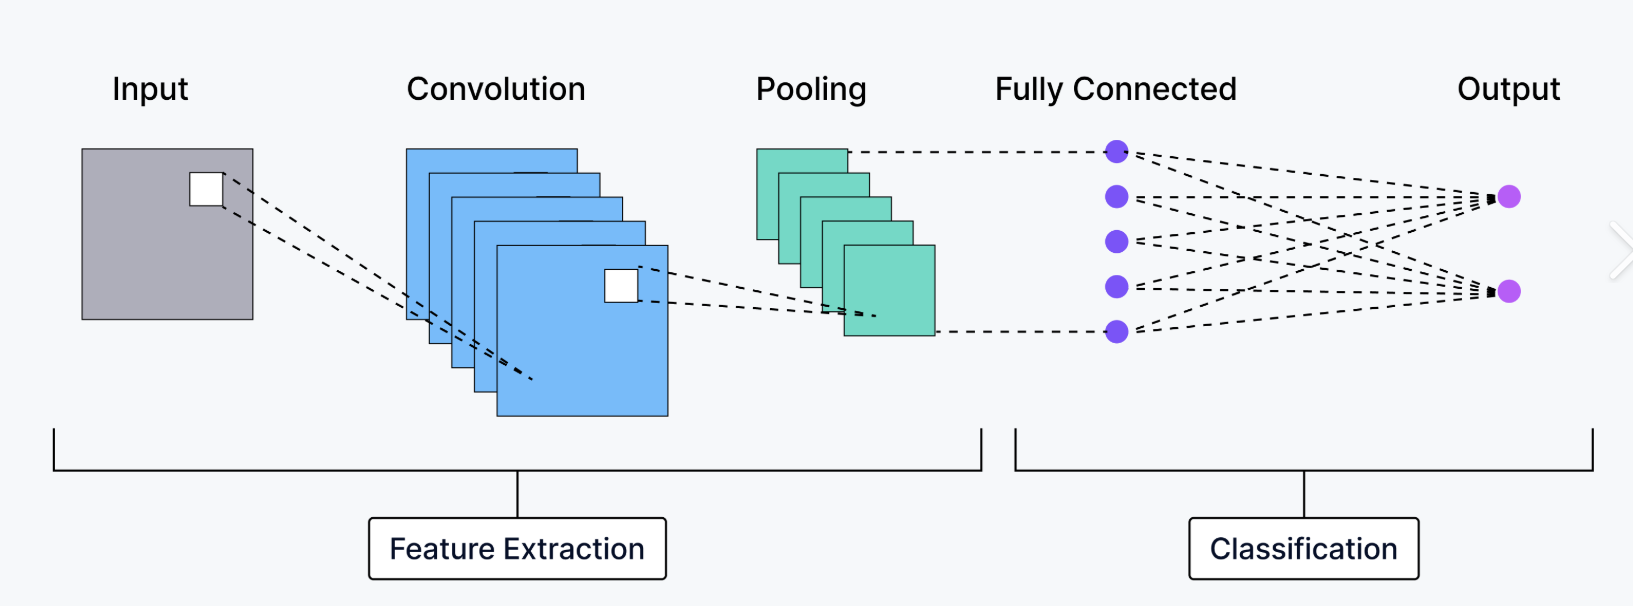
\includegraphics[width=0.8\textwidth]{figChap1/CNN_kien_truc.png}
    \caption{Kiến trúc cơ bản của Mạng Nơ-ron Tích chập}
    \label{fig:cnn_basic}
\end{figure}

\subsection{Lớp Tích chập, Pooling và Hàm kích hoạt}

\textbf{Lớp tích chập} sử dụng các kernel nhỏ (thường $3 \times 3$) trượt trên ảnh đầu vào, thực hiện phép nhân tích chập cục bộ để trích xuất các đặc trưng hình học như cạnh, đường cong và kết cấu. Mỗi kernel được học tự động trong quá trình huấn luyện, thay thế hoàn toàn các đặc trưng thủ công (SIFT, HOG) của thị giác máy tính truyền thống \cite{Basha2020, Girshick2014}.

\textbf{Lớp Pooling} (thường là Max Pooling) giảm độ phân giải không gian của bản đồ đặc trưng, giúp giảm chi phí tính toán và tạo tính bất biến dịch chuyển cục bộ. Tuy nhiên, pooling gây mất thông tin vị trí chính xác -- một hạn chế cần được xử lý trong các tác vụ yêu cầu độ chính xác pixel như sinh ảnh \cite{Basha2020}.

\textbf{Hàm kích hoạt} đưa tính phi tuyến vào mạng. Trong các kiến trúc GAN hiện đại, hai hàm được sử dụng phổ biến nhất là \cite{Nair2010, Maas2013}:
\begin{itemize}
    \item \textbf{ReLU} ($\max(0, x)$): Tiêu chuẩn cho hầu hết CNN, giảm vanishing gradient nhưng có thể gây ``Dying ReLU'' khi nơ-ron nhận giá trị âm liên tục.
    \item \textbf{Leaky ReLU} ($\max(\alpha x, x)$ với $\alpha = 0.01$): Khắc phục Dying ReLU bằng cách giữ gradient nhỏ cho giá trị âm. Được sử dụng rộng rãi trong Generator và Discriminator của AnimeGANv3 \cite{Liu2024}.
\end{itemize}

\begin{figure}[H]
    \centering
    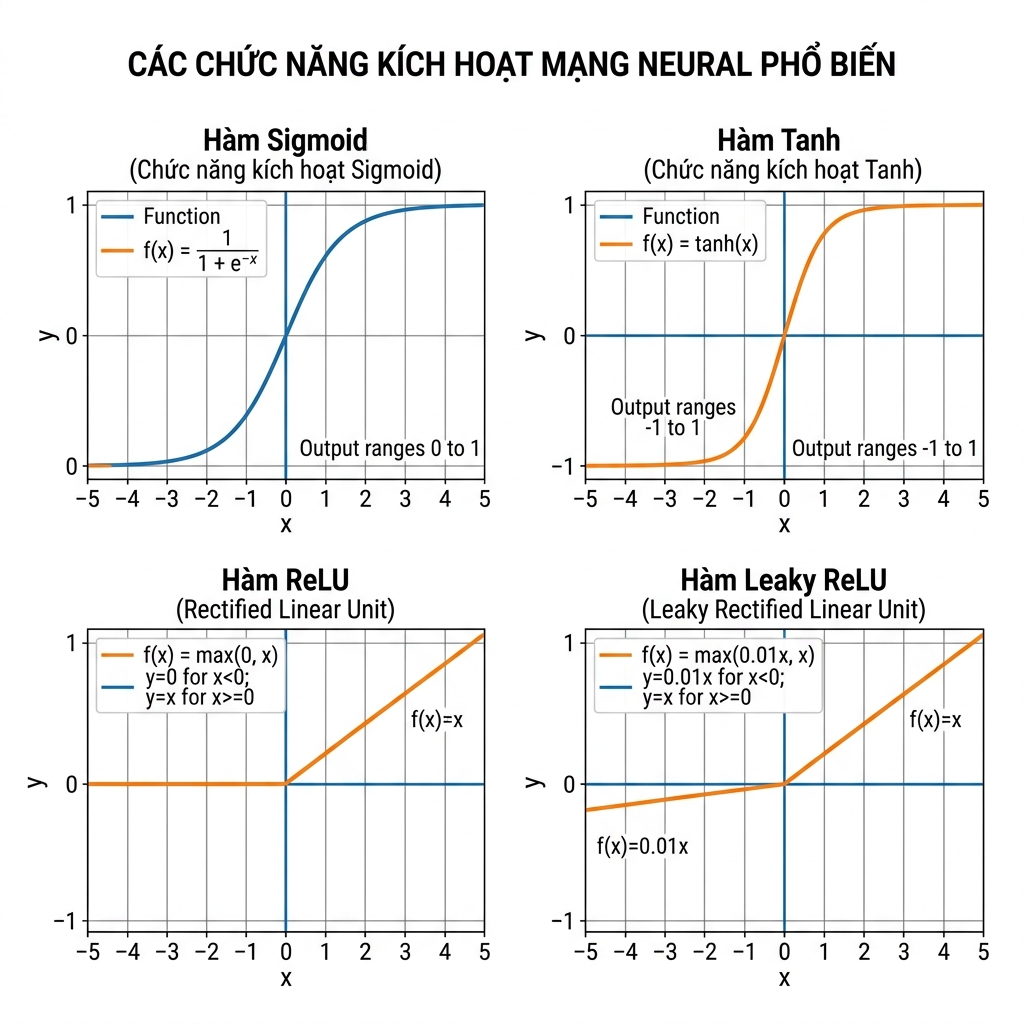
\includegraphics[width=0.75\textwidth]{figChap1/activation_functions.png}
    \caption{So sánh các hàm kích hoạt: Sigmoid, Tanh, ReLU và Leaky ReLU}
    \label{fig:activation_functions}
\end{figure}

\subsection{Các Kỹ thuật Chuẩn hóa}
\label{subsec:normalization}

Chuẩn hóa (Normalization) là cơ chế thiết yếu để ổn định và tăng tốc quá trình huấn luyện mạng sâu. Bốn kỹ thuật chính được phân biệt theo chiều tính toán thống kê trên tensor đặc trưng $(N \times C \times H \times W)$:

\begin{itemize}
    \item \textbf{Batch Normalization (BN)} \cite{Ioffe2015}: Chuẩn hóa theo chiều batch $N$, giảm Internal Covariate Shift. Nhạy cảm với kích thước batch nhỏ.
    \item \textbf{Layer Normalization (LN)} \cite{Ba2016}: Chuẩn hóa toàn bộ kênh $C$ của một mẫu. Phổ biến trong Transformers và RNNs.
    \item \textbf{Group Normalization (GN)} \cite{Wu2018}: Chia kênh thành nhóm nhỏ, cân bằng giữa BN và IN. Không phụ thuộc batch size.
    \item \textbf{Instance Normalization (IN)} \cite{Ulyanov2016}: Chuẩn hóa từng kênh của từng mẫu độc lập. \textbf{Đặc biệt quan trọng} cho bài toán chuyển phong cách vì IN loại bỏ thông tin phong cách toàn cục, cho phép mô hình học phong cách mới. IN là nền tảng trực tiếp của kỹ thuật LADE trong AnimeGANv3 (trình bày ở Chương~2).
\end{itemize}

\begin{figure}[H]
    \centering
    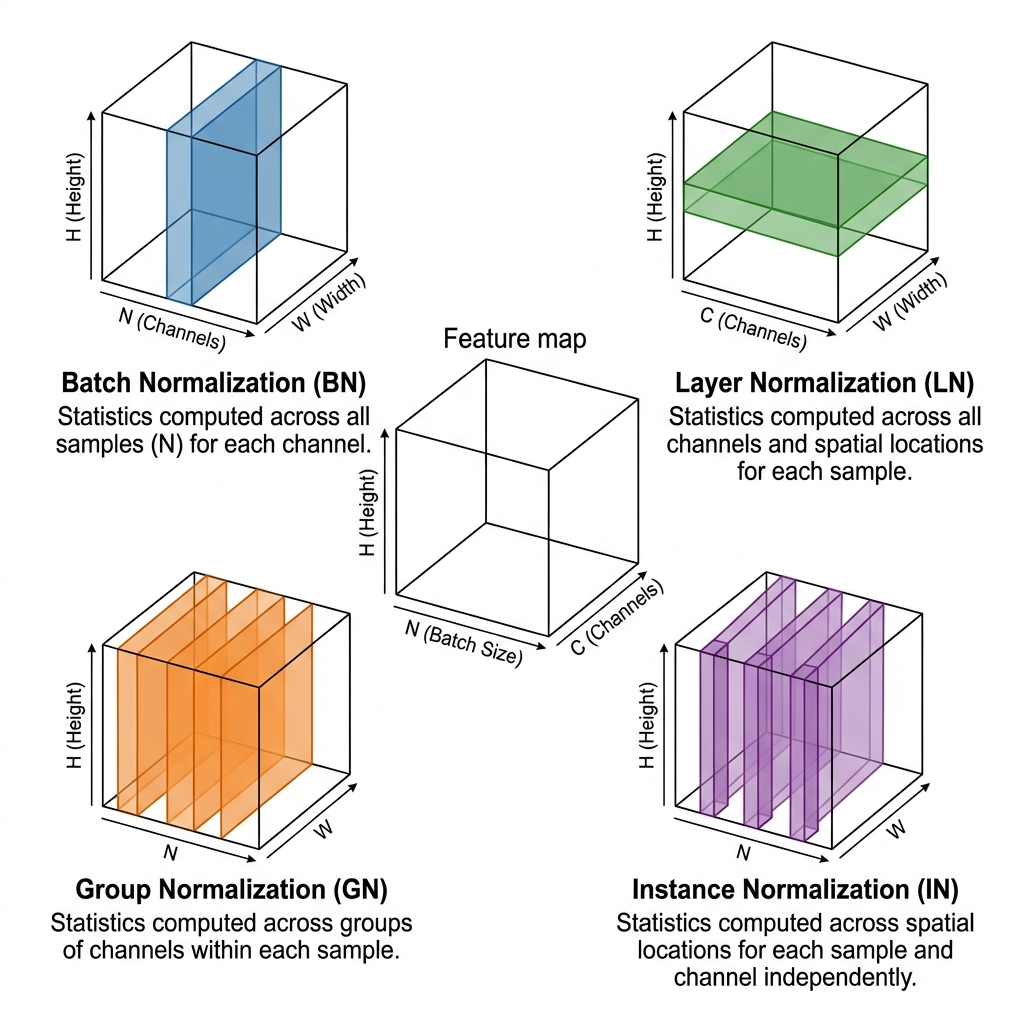
\includegraphics[width=0.85\textwidth]{figChap1/normalization_comparison.png}
    \caption{So sánh bốn kỹ thuật chuẩn hóa trên tensor $(N \times C \times H \times W)$}
    \label{fig:normalization_comparison}
\end{figure}
    \noindent\textit{Chú thích:} BN chuẩn hóa theo chiều batch $N$; LN theo toàn bộ kênh $C$ của một mẫu; GN theo nhóm kênh; IN theo từng kênh của từng mẫu độc lập \cite{Wu2018, Ulyanov2016}

Ngoài ra, \textbf{Spectral Normalization (SN)} \cite{Miyato2018} chuẩn hóa ma trận trọng số $W$ bằng cách chia cho giá trị kỳ dị lớn nhất $\sigma(W)$, đảm bảo ràng buộc Lipschitz cho Discriminator. SN đã trở thành tiêu chuẩn trong hầu hết kiến trúc GAN hiện đại \cite{Zhang2019, Brock2018}.

\subsection{Kiến trúc Encoder-Decoder}
\label{subsec:encoder_decoder}

Kiến trúc Encoder-Decoder là nền tảng cho các bài toán dịch ảnh (image-to-image translation). Phần \textbf{Encoder} sử dụng tích chập và downsampling để nén ảnh gốc thành vector đặc trưng ẩn, trong khi phần \textbf{Decoder} tái tạo vector ẩn thành ảnh đầu ra mong muốn \cite{Hasan2019}.

\begin{figure}[H]
    \centering
    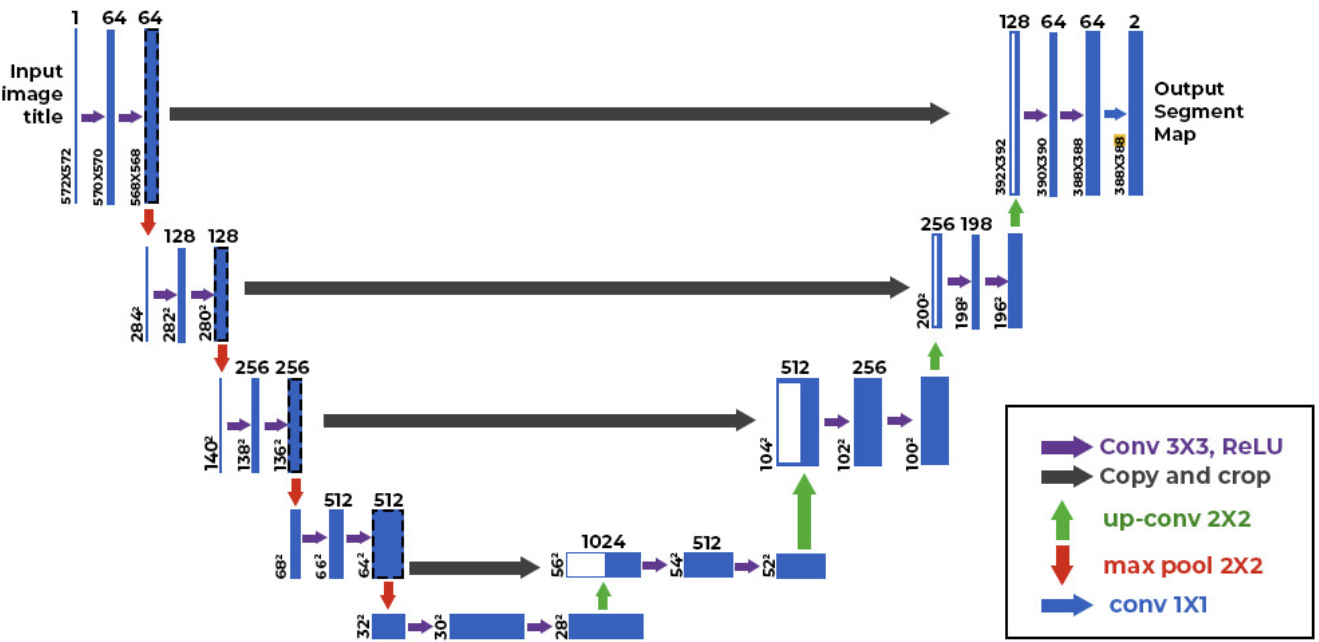
\includegraphics[width=0.9\textwidth]{figChap1/u-net.png}
    \caption{Kiến trúc U-Net với skip connections}
    \label{fig:u-net}
\end{figure}

Biến thể U-Net bổ sung \textbf{skip connections} kết nối trực tiếp giữa các tầng encoder và decoder cùng độ phân giải. Cơ chế này cho phép decoder truy cập đặc trưng chi tiết cục bộ từ encoder, khắc phục hiện tượng mất thông tin không gian qua bottleneck \cite{Hasan2019}. Generator trong AnimeGANv3 sử dụng kiến trúc U-Net cho cả hai nhánh decoder (Chương~2).

Trong phần decoder, việc tăng độ phân giải (upsampling) có hai lựa chọn chính:
\begin{itemize}
    \item \textbf{Transposed Convolution}: Lớp học được, nhưng dễ gây lỗi đồ họa dạng checkerboard do chồng lấp không đều \cite{Hasan2019}.
    \item \textbf{Bilinear/Nearest-Neighbor Interpolation + Conv}: Không học được phần upsampling, nhưng loại bỏ lỗi đồ họa dạng checkerboard. AnimeGANv3 chọn phương pháp này để đảm bảo ảnh đầu ra mịn \cite{Liu2024}.
\end{itemize}

% =====================================================
\section{Kiến trúc Mạng Đối nghịch Tạo sinh}
\label{sec:gan}

Mạng Đối nghịch Tạo sinh (Generative Adversarial Networks -- GANs) do Ian Goodfellow và cộng sự đề xuất năm 2014 \cite{Goodfellow2014} là nền tảng cho hầu hết các phương pháp chuyển đổi phong cách ảnh hiện đại. Khác với các mô hình tạo sinh trước đây dựa trên phương pháp xác suất phức tạp, GAN sử dụng trò chơi đối kháng giữa hai mạng nơ-ron để tạo ra dữ liệu có độ trung thực cao.

\subsection{Nguyên lý Hoạt động và Hàm Mục tiêu}
\subsubsection{Khung Làm việc Đối kháng}

GAN gồm hai mạng nơ-ron được huấn luyện đồng thời qua trò chơi có tổng bằng không \cite{Goodfellow2014}:
\begin{itemize}
    \item \textbf{Generator (G):} Nhận vector nhiễu ngẫu nhiên $z \sim p_z(z)$ từ không gian tiềm ẩn và tạo ra mẫu giả $G(z)$. Mục tiêu: đánh lừa Discriminator.
    \item \textbf{Discriminator (D):} Bộ phân loại nhị phân, nhận dữ liệu $x$ và xuất xác suất $D(x)$ dữ liệu đó là thật. Mục tiêu: phân biệt dữ liệu thật và giả.
\end{itemize}

\begin{figure}[H]
    \centering
    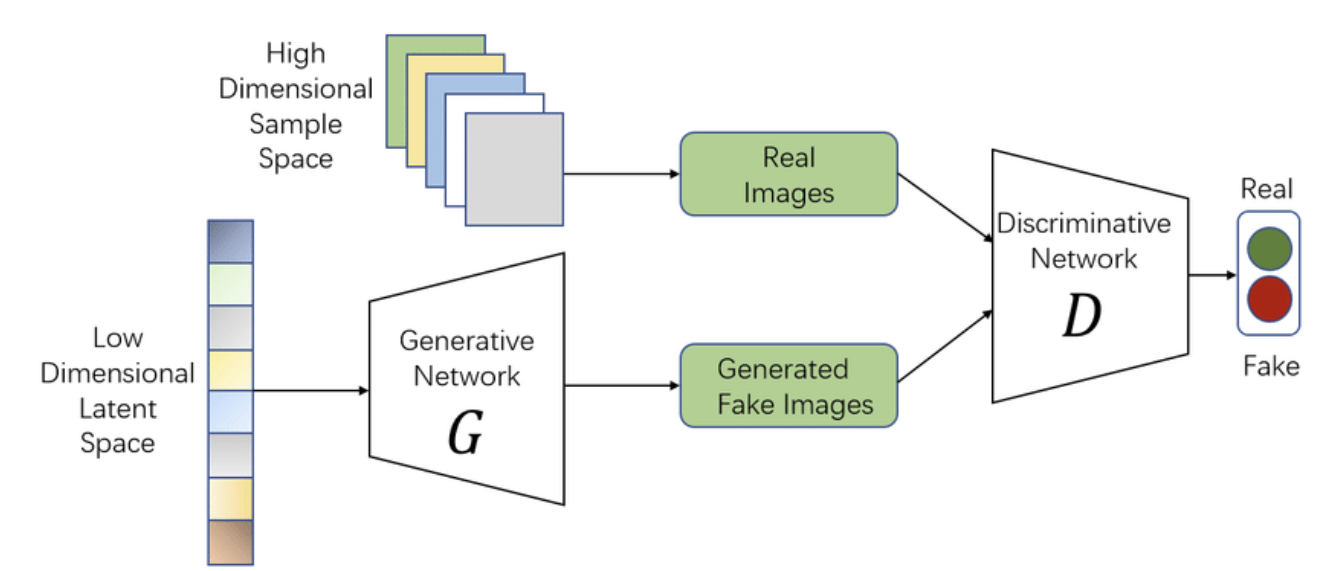
\includegraphics[width=0.85\textwidth]{figChap1/gan-architect.png}
    \caption{Kiến trúc tổng quát của Mạng Đối nghịch Tạo sinh (GAN)}
    \label{fig:gan}
\end{figure}
    \noindent\textit{Chú thích:} Generator $G$ nhận vector nhiễu $z \sim p_z(z)$ để tạo mẫu giả $G(z)$, Discriminator $D$ phân biệt dữ liệu thật $x$ với dữ liệu giả. Hai mạng huấn luyện đồng thời theo trò chơi minimax \cite{Goodfellow2014}

\subsubsection{Trò chơi Minimax}

Quá trình huấn luyện được mô hình hóa dưới dạng bài toán tối ưu Minimax \cite{Goodfellow2014}:
\begin{equation}
\label{eq:gan_minimax}
\min_G \max_D V(D, G) = \underbrace{\mathbb{E}_{x \sim p_{\text{data}}(x)}[\log D(x)]}_{\text{(1) Discriminator nhận dạng ảnh thật}} + \underbrace{\mathbb{E}_{z \sim p_z(z)}[\log(1 - D(G(z)))]}_{\text{(2) Discriminator bác bỏ ảnh giả}}
\end{equation}

\noindent trong đó:
\begin{itemize}
    \item $G: \mathcal{Z} \rightarrow \mathcal{X}$ -- Generator ánh xạ vector nhiễu $z$ từ không gian tiềm ẩn $\mathcal{Z}$ sang không gian ảnh $\mathcal{X}$.
    \item $D: \mathcal{X} \rightarrow [0,1]$ -- Discriminator xuất xác suất mẫu đầu vào là ảnh thật.
    \item $p_{\text{data}}(x)$ -- phân phối dữ liệu thật; $p_z(z)$ -- phân phối nhiễu đầu vào (thường là $\mathcal{N}(0,I)$).
    \item $\mathbb{E}[\cdot]$ -- kỳ vọng thống kê trên phân phối tương ứng.
\end{itemize}

\textbf{Ý nghĩa từng số hạng:}
\begin{itemize}
    \item \textbf{Số hạng (1)} $\mathbb{E}[\log D(x)]$: Với mẫu thật $x \sim p_{\text{data}}$, $D(x)$ càng gần 1 thì $\log D(x)$ càng gần 0 (lớn nhất). Discriminator muốn \textit{tối đa hóa} số hạng này -- tức là gán xác suất cao cho ảnh thật.
    \item \textbf{Số hạng (2)} $\mathbb{E}[\log(1 - D(G(z)))]$: Với mẫu giả $G(z)$, nếu Discriminator nhận ra giả thì $D(G(z)) \approx 0$, khiến $\log(1-D(G(z))) \approx 0$ (lớn nhất). Generator muốn \textit{tối thiểu hóa} số hạng này -- tức là đánh lừa $D$ bằng cách làm $D(G(z)) \rightarrow 1$.
\end{itemize}

\subsubsection{Điểm Cân bằng Nash và Discriminator Tối ưu}

Mục tiêu cuối cùng là đạt \textit{Điểm cân bằng Nash}, nơi $D$ không thể phân biệt ảnh thật và giả ($D(x) = 0.5$ cho mọi $x$), và phân phối sinh $p_g$ trùng khớp với $p_{\text{data}}$ \cite{Jabbar2021}. Với $G$ cố định, Discriminator tối ưu theo $V(D,G)$ là:
\begin{equation}
\label{eq:discriminator_optimal}
D^*_G(x) = \frac{p_{\text{data}}(x)}{p_{\text{data}}(x) + p_g(x)}
\end{equation}

\noindent trong đó $p_g(x)$ là phân phối của mẫu giả $G(z)$ khi $z \sim p_z$. Công thức này có thể giải tích bằng cách lấy đạo hàm $\frac{\partial V}{\partial D(x)} = 0$: tại mỗi điểm $x$, $D^*$ cân bằng tỷ lệ giữa mật độ thật và tổng mật độ. Khi $p_g = p_{\text{data}}$, ta có $D^*(x) = \tfrac{1}{2}$ -- Discriminator không thể làm tốt hơn đoán ngẫu nhiên.

Thay $D^*_G$ vào Phương trình~(\ref{eq:gan_minimax}), hàm mục tiêu của Generator rút gọn thành:
\begin{equation}
\label{eq:generator_jsd}
C(G) = -\log 4 + 2 \cdot D_{\text{JS}}(p_{\text{data}} \,\|\, p_g)
\end{equation}

\noindent trong đó $D_{\text{JS}}(p \,\|\, q) = \frac{1}{2} D_{\text{KL}}\!\left(p \,\Big\|\, \frac{p+q}{2}\right) + \frac{1}{2} D_{\text{KL}}\!\left(q \,\Big\|\, \frac{p+q}{2}\right)$ là khoảng cách Jensen-Shannon -- phiên bản đối xứng của phân kỳ KL. Vì $D_{\text{JS}} \geq 0$ và bằng 0 khi và chỉ khi $p_{\text{data}} = p_g$, hàm $C(G)$ đạt cực tiểu toàn cục tại $C^* = -\log 4$ đúng khi Generator tái tạo hoàn hảo phân phối dữ liệu thật.


\subsection{Thách thức trong Huấn luyện GAN}
\label{subsec:gan_challenges}

Mặc dù lý thuyết Minimax chặt chẽ, GAN trong thực tế gặp ba vấn đề nghiêm trọng \cite{Salimans2016, Heusel2017}. Các vấn đề này bắt nguồn từ sự không tương thích giữa giả định toán học (phân phối liên tục, tập dữ liệu vô hạn) và thực tế huấn luyện (mini-batch hữu hạn, không gian ảnh chiều cao).

\subsubsection{Biến mất Gradient (Vanishing Gradients)}

Trong không gian ảnh chiều cao, $p_{\text{data}}$ và $p_g$ thường tập trung trên các đa tạp (manifold) chiều thấp không giao nhau. Khi đó, tồn tại siêu phẳng hoàn toàn tách hai phân phối và Discriminator tối ưu đạt độ chính xác 100\% \cite{Arjovsky2017}.

\textbf{Phân tích toán học:} Khi $p_{\text{data}}$ và $p_g$ tách rời hoàn toàn (disjoint support), Discriminator tối ưu $D^*(x) = 1$ với $x \sim p_{\text{data}}$ và $D^*(x) = 0$ với $x \sim p_g$. Thay vào hàm $C(G)$ (Phương trình~\ref{eq:generator_jsd}):
\begin{equation}
\label{eq:jsd_disjoint}
D_{\text{JS}}(p_{\text{data}} \,\|\, p_g) = \log 2 \quad \Rightarrow \quad C(G) = -\log 4 + 2\log 2 = 0
\end{equation}
Gradient $\nabla_\theta C(G)$ bằng 0 với mọi tham số $\theta$ của Generator -- mạng hoàn toàn không nhận được tín hiệu học.

\textbf{Biểu hiện thực tế:} Đường cong $G\_\text{loss}$ của Generator phẳng lặng trong khi $D\_\text{loss}$ giảm về 0. Ảnh sinh ra không cải thiện theo epoch dù loss Discriminator tiếp tục tối ưu hóa.

\subsubsection{Sụp đổ Mode (Mode Collapse)}
\label{subsubsec:mode_collapse}

Mode Collapse xảy ra khi Generator tìm được một hoặc vài ``chiến lược an toàn'' -- tức là một tập mẫu nhỏ có thể đánh lừa Discriminator hiện tại -- và cố định vào đó thay vì học toàn bộ phân phối $p_{\text{data}}$.

\textbf{Cơ chế game-theoretic:} Quá trình huấn luyện GAN là trò chơi hai người với chiến lược thay đổi theo thời gian. Khi Generator ``chuyên môn hóa'' vào mode $m^*$:
\begin{equation}
\label{eq:mode_collapse_dynamics}
G_t(z) \approx m^* \;\forall z \quad \Rightarrow \quad D_{t+1} \text{ học phân biệt } m^* \quad \Rightarrow \quad G_{t+2} \text{ chuyển sang mode khác } m^{**}
\end{equation}
Hai mạng đuổi bắt nhau theo vòng tròn: Generator liên tục ``bỏ trốn'' sang mode mới, Discriminator liên tục ``học đuổi'', nhưng không bao giờ đạt cân bằng Nash toàn cục.

\textbf{Hậu quả định lượng:} Với bộ dữ liệu có $K$ mode (ví dụ: $K$ phong cách anime), Generator bị collapse thường chỉ bao phủ $1$--$3$ mode, dẫn đến FID cao do phân phối sinh thiếu đa dạng \cite{Salimans2016}.

\begin{figure}[H]
    \centering
    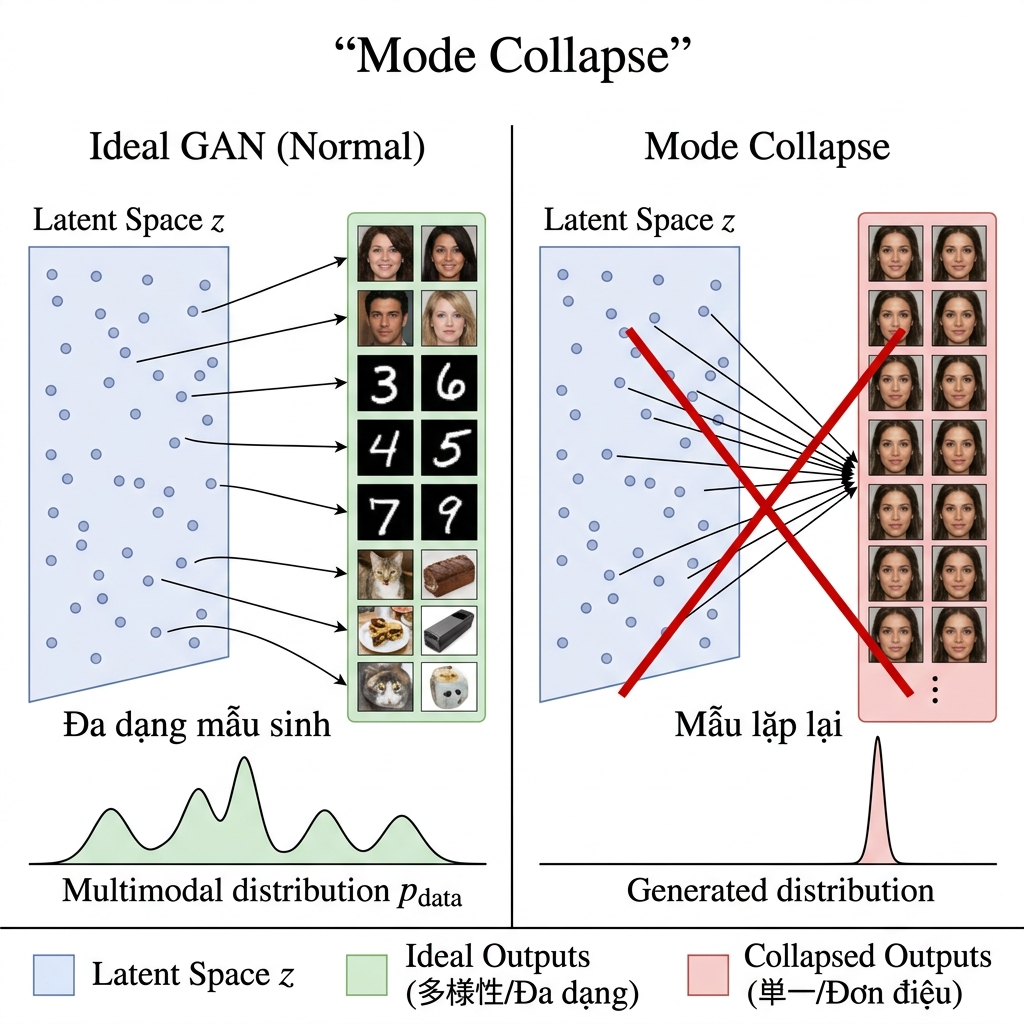
\includegraphics[width=0.95\textwidth]{figChap1/mode_collapse.png}
    \caption{Minh họa hiện tượng Mode Collapse trong GAN}
    \label{fig:mode_collapse}
\end{figure}
    \noindent\textit{Chú thích:} (Trái) GAN lý tưởng: không gian $z$ đa dạng ánh xạ sang nhiều mode của $p_{\text{data}}$. (Phải) Mode Collapse: toàn bộ không gian $z$ bị ánh xạ vào một hoặc vài mode duy nhất, phần còn lại của phân phối không được học \cite{Salimans2016}.

\subsubsection{Không Hội tụ (Non-Convergence)}
\label{subsubsec:non_convergence}

GAN yêu cầu tìm \textit{điểm yên ngựa} (saddle point) $(\theta_G^*, \theta_D^*)$ thoả mãn $\min_G \max_D V(D,G)$, không phải cực tiểu thông thường. Tuy nhiên, gradient descent tiêu chuẩn được thiết kế để tìm cực tiểu cục bộ -- đây là sự không tương thích cơ bản \cite{Heusel2017}.

\textbf{Ví dụ minh họa (Bilinear Game):} Xét trò chơi đơn giản nhất với $V(x, y) = xy$, tương tự bài toán GAN:
\begin{equation}
\label{eq:bilinear_game}
\dot{x} = -\frac{\partial V}{\partial x} = -y, \qquad \dot{y} = +\frac{\partial V}{\partial y} = x
\end{equation}
Nghiệm của hệ này là $x(t) = r\cos(t + \phi)$, $y(t) = r\sin(t + \phi)$ -- quỹ đạo \textit{xoay tròn vĩnh viễn} với bán kính $r$ không đổi, không bao giờ hội tụ về điểm cân bằng $(0,0)$.

\textbf{Biểu hiện thực tế:} $G\_\text{loss}$ và $D\_\text{loss}$ dao động có chu kỳ thay vì giảm đơn điệu. Trong GAN huấn luyện ổn định, dao động nhỏ là bình thường; dao động lớn theo chu kỳ ($> 20\%$ biên độ tương đối) là dấu hiệu non-convergence nghiêm trọng.

\begin{figure}[H]
    \centering
    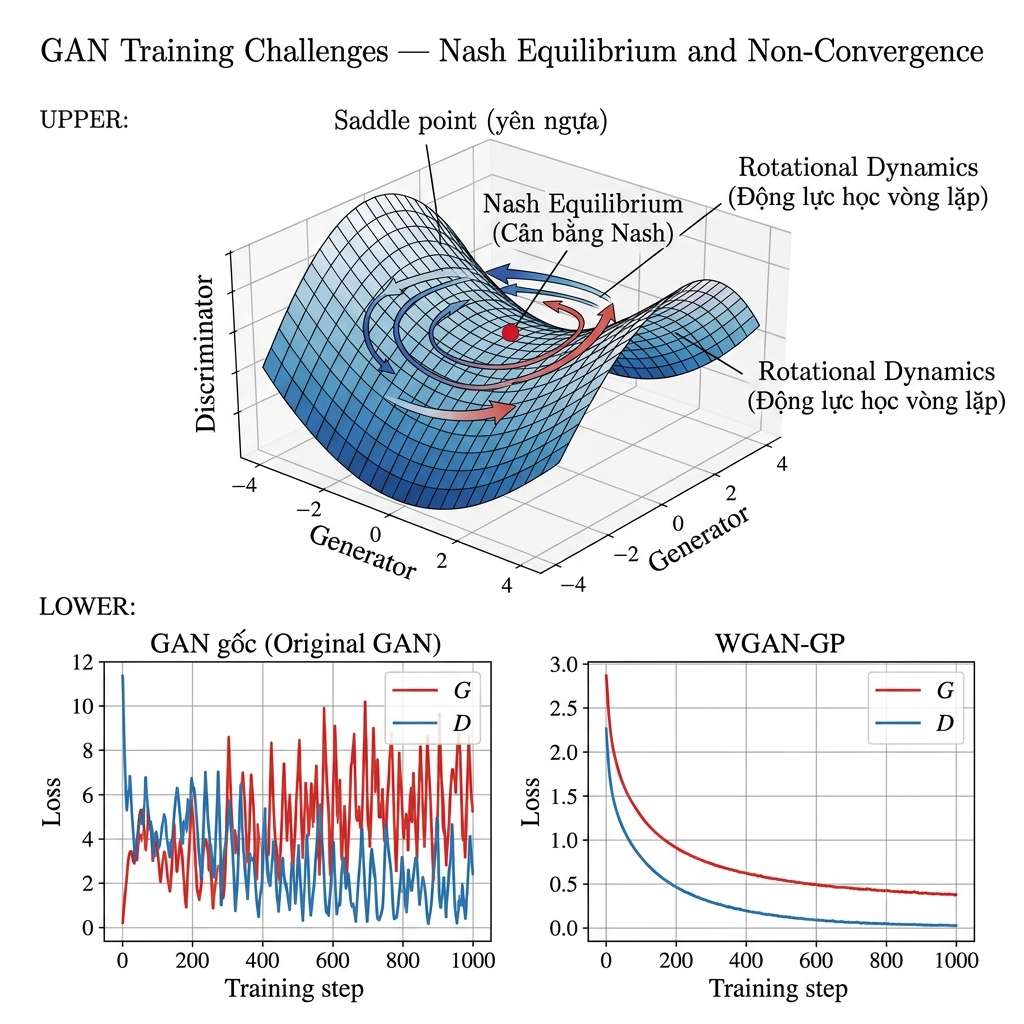
\includegraphics[width=0.75\textwidth]{figChap1/nash_equilibrium.png}
    \caption{Động lực học huấn luyện GAN: quỹ đạo xoay tròn trong không gian tham số và vấn đề Không Hội tụ}
    \label{fig:nash_equilibrium}
\end{figure}
    \noindent\textit{Chú thích:} Mũi tên thể hiện hướng cập nhật gradient của $(\theta_G, \theta_D)$ tại mỗi bước. Thay vì hội tụ vào tâm (điểm cân bằng Nash), quỹ đạo xoay theo đường tròn -- đặc trưng của saddle-point dynamics.

\begin{longtable}{>{\bfseries}m{3.5cm} | m{4.2cm} | m{4.2cm} | m{3.1cm}}
\caption{Tóm tắt các chế độ thất bại của GAN và giải pháp tương ứng}
\label{tab:gan_failure_modes} \\
\toprule
Vấn đề & Biểu hiện & Nguyên nhân Toán học & Giải pháp Tiêu biểu \\
\midrule
\endhead
Vanishing Gradients & $G$ ngừng học, $G\_\text{loss}$ phẳng & $D^*$ tách hoàn toàn hai phân phối, $D_{\text{JS}} = \log 2$, gradient $= 0$ & WGAN \cite{Arjovsky2017} dùng khoảng cách Wasserstein \\
\midrule
Mode Collapse & Ảnh sinh ra giống hệt nhau, FID cao & $G$ tối ưu hóa cục bộ, đuổi bắt vòng tròn qua các mode & Minibatch discrimination, Unrolled GAN \cite{Salimans2016} \\
\midrule
Non-Convergence & Loss dao động mạnh theo chu kỳ & Saddle-point dynamics, gradient descent không hội tụ & WGAN-GP \cite{Gulrajani2017}, Spectral Norm \cite{Miyato2018} \\
\bottomrule
\end{longtable}


\subsection{Các Giải pháp về Hàm Mục tiêu}

\subsubsection{Wasserstein GAN (WGAN)}
\label{subsubsec:wgan}

Arjovsky et al.~\cite{Arjovsky2017} phân tích nguyên nhân gốc rễ của Vanishing Gradients: khoảng cách Jensen-Shannon không liên tục khi hai phân phối không giao nhau. Giải pháp là thay thế bằng \textit{khoảng cách Wasserstein-1} (Earth-Mover distance):
\begin{equation}
\label{eq:wasserstein}
W(p_{\text{data}}, p_g) = \inf_{\gamma \in \Pi(p_{\text{data}}, p_g)} \mathbb{E}_{(x,y) \sim \gamma} \left[ \|x - y\| \right]
\end{equation}

\noindent trong đó $\Pi(p_{\text{data}}, p_g)$ là tập tất cả phân phối ghép cặp (joint distributions) với marginal $p_{\text{data}}$ và $p_g$. Trực quan, $W$ đo lượng ``đất'' tối thiểu cần di chuyển để biến $p_g$ thành $p_{\text{data}}$. Không giống $D_{\text{JS}}$, $W$ vẫn liên tục ngay cả khi hai phân phối hoàn toàn không giao nhau.

\textbf{Dạng đối ngẫu Kantorovich--Rubinstein:} Vì Phương trình~(\ref{eq:wasserstein}) khó tính trực tiếp, WGAN sử dụng dạng tương đương:
\begin{equation}
\label{eq:wgan_dual}
W(p_{\text{data}}, p_g) = \frac{1}{K} \sup_{\|f\|_L \leq K} \left( \mathbb{E}_{x \sim p_{\text{data}}}[f(x)] - \mathbb{E}_{\tilde{x} \sim p_g}[f(\tilde{x})] \right)
\end{equation}

\noindent trong đó $\sup$ lấy trên tất cả hàm $K$-Lipschitz $f: \mathcal{X} \rightarrow \mathbb{R}$. Discriminator $D_w$ đóng vai trò xấp xỉ hàm $f$ này thay vì phân loại nhị phân, và hàm mục tiêu WGAN là:
\begin{equation}
\label{eq:wgan_objective}
\min_G \max_{D_w \in \mathcal{F}_1} \; \mathbb{E}_{x \sim p_{\text{data}}}[D_w(x)] - \mathbb{E}_{z \sim p_z}[D_w(G(z))]
\end{equation}

\noindent với $\mathcal{F}_1$ là lớp hàm 1-Lipschitz. Ràng buộc Lipschitz là điều kiện bắt buộc để đảm bảo supremum hữu hạn và gradient không bùng nổ. Trong bản gốc WGAN, ràng buộc này được áp đặt bằng \textit{Weight Clipping}: sau mỗi bước cập nhật, trọng số $w$ bị clamp về $[-c, c]$ (thường $c = 0.01$).

\begin{figure}[H]
    \centering
    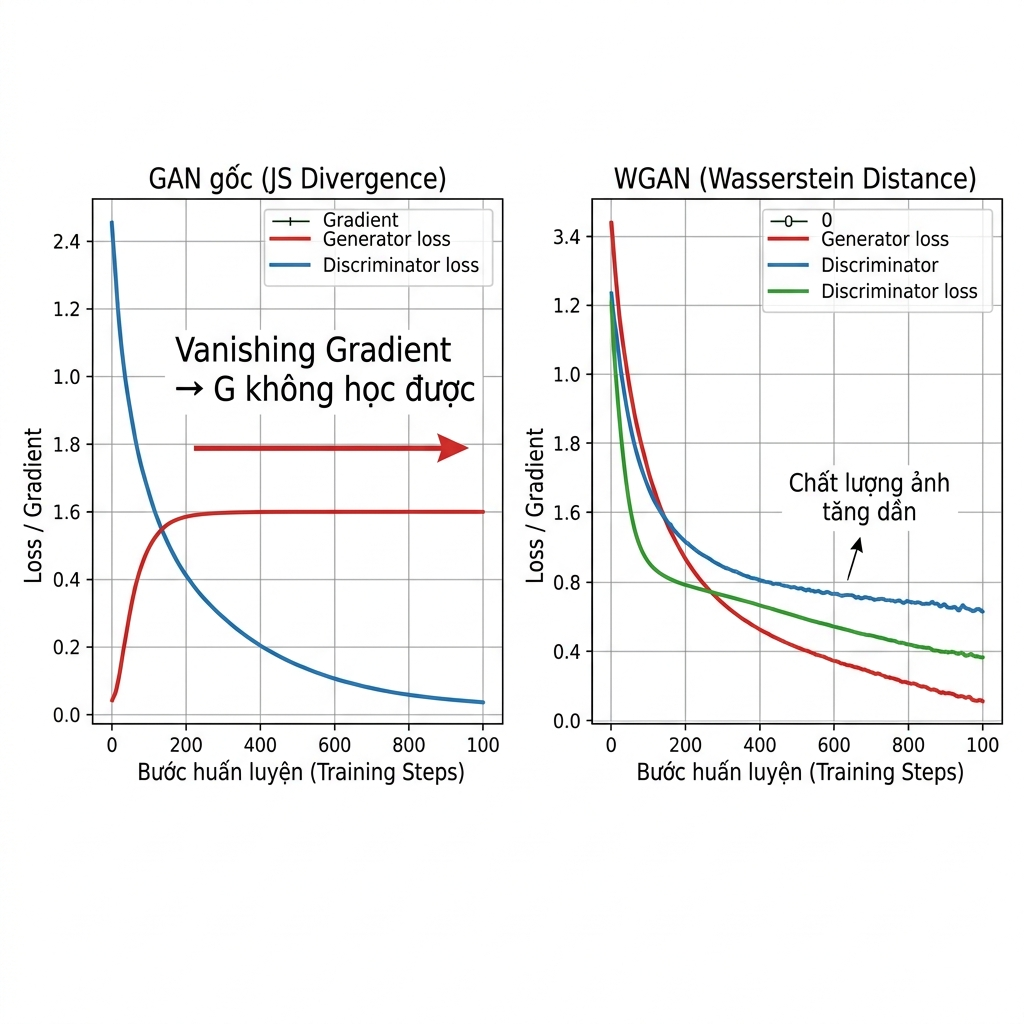
\includegraphics[width=0.8\textwidth]{figChap1/wgan_vs_gan_gradient.png}
    \caption{So sánh gradient flow giữa GAN gốc (JS divergence) và WGAN (Wasserstein distance) khi hai phân phối không giao nhau}
    \label{fig:wgan_vs_gan}
\end{figure}
    \noindent\textit{Chú thích:} (Trái) GAN gốc: khi $p_g$ không giao với $p_{\text{data}}$, $D_{\text{JS}} = \log 2$ hằng số, gradient Generator bằng 0. (Phải) WGAN: khoảng cách Wasserstein vẫn tuyến tính theo khoảng cách giữa hai phân phối, cung cấp gradient có hướng rõ ràng \cite{Arjovsky2017}.

\subsubsection{WGAN-GP: Gradient Penalty}
\label{subsubsec:wgan_gp}

Weight Clipping trong WGAN gốc gây ra hai vấn đề: (1) mô hình bị ``underfit'' do không gian hàm bị giới hạn quá chặt, và (2) gradient bùng nổ hoặc biến mất do trọng số tập trung về $\pm c$. Gulrajani et al.~\cite{Gulrajani2017} giải quyết bằng cách thay thế bằng \textit{Gradient Penalty} -- phạt trực tiếp trên norm gradient:

\begin{equation}
\label{eq:wgan_gp}
L_{\text{WGAN-GP}} =
\underbrace{\mathbb{E}_{\tilde{x} \sim p_g}[D(\tilde{x})] - \mathbb{E}_{x \sim p_{\text{data}}}[D(x)]}_{\text{(1) WGAN critic loss}} 
+
\underbrace{\lambda \, \mathbb{E}_{\hat{x} \sim p_{\hat{x}}}\!\left[\left(\|\nabla_{\hat{x}} D(\hat{x})\|_2 - 1\right)^2\right]}_{\text{(2) Gradient Penalty}}
\end{equation}

\noindent trong đó:
\begin{itemize}
    \item $\tilde{x} = G(z)$ -- mẫu giả từ Generator; $x$ -- mẫu thật từ $p_{\text{data}}$.
    \item $\hat{x} = \epsilon x + (1-\epsilon)\tilde{x}$, $\epsilon \sim \mathcal{U}[0,1]$ -- điểm nội suy ngẫu nhiên giữa mẫu thật và giả, được lấy mẫu dọc theo đường thẳng nối hai phân phối.
    \item $\lambda = 10$ -- hệ số cân bằng giữa critic loss và penalty (giá trị mặc định theo \cite{Gulrajani2017}).
    \item Số hạng $(2)$: phạt khi $\|\nabla_{\hat{x}} D(\hat{x})\|_2 \neq 1$, ép Discriminator thỏa mãn điều kiện 1-Lipschitz tại các điểm quan trọng nhất (trên ``straight-line path'' giữa hai phân phối).
\end{itemize}

\textbf{Ưu điểm so với Weight Clipping:} GP không giới hạn cứng không gian tham số, cho phép Discriminator học các hàm phức tạp hơn. Thực nghiệm cho thấy WGAN-GP hội tụ nhanh hơn và ổn định hơn trên các kiến trúc ResNet sâu \cite{Gulrajani2017}.

\subsubsection{Spectral Normalization (SN-GAN)}
\label{subsubsec:sn_gan}

Miyato et al.~\cite{Miyato2018} đề xuất cách áp đặt ràng buộc Lipschitz nhẹ nhàng hơn bằng cách chuẩn hóa ma trận trọng số theo \textit{spectral norm} (giá trị kỳ dị lớn nhất):
\begin{equation}
\label{eq:spectral_norm}
W_{\text{SN}} = \frac{W}{\sigma(W)}, \qquad \sigma(W) = \max_{\|u\|=1} \|Wu\|_2
\end{equation}

\noindent trong đó $\sigma(W)$ là giá trị kỳ dị lớn nhất (singular value) của $W$, tính hiệu quả bằng \textit{power iteration} chỉ một bước mỗi lần cập nhật. Sau chuẩn hóa, hằng số Lipschitz của từng lớp tuyến tính bị giới hạn:
\begin{equation}
\label{eq:lipschitz_sn}
\|W_{\text{SN}} u\|_2 \leq \|u\|_2 \quad \forall u \quad \Rightarrow \quad \text{Lip}(W_{\text{SN}}) \leq 1
\end{equation}

Áp dụng cho mọi lớp trong Discriminator, ràng buộc Lipschitz toàn cục được đảm bảo qua quy tắc nhân: $\text{Lip}(D) \leq \prod_l \sigma(W_l) = 1$. \textbf{Ưu điểm chính:} chi phí tính toán gần như không đổi (chỉ thêm một lần power iteration), không cần điều chỉnh hyperparameter như $\lambda$ của GP. Spectral Normalization được sử dụng trực tiếp trong Discriminator của AnimeGANv3 \cite{Liu2024} (phân tích chi tiết tại Mục~2.4).

\subsubsection{Least Squares GAN (LSGAN)}
\label{subsubsec:lsgan}

Mao et al.~\cite{Mao2017} chỉ ra vấn đề khác của cross-entropy: ngay cả khi mẫu giả $G(z)$ nằm ở đúng phía phân loại nhưng còn xa decision boundary, loss đã bão hòa và không cung cấp gradient để đẩy mẫu về phía dữ liệu thật. LSGAN thay thế cross-entropy bằng \textit{bình phương sai số} (least squares):

\begin{align}
\label{eq:lsgan_D}
\mathcal{L}_{\text{adv}}^D &= \frac{1}{2}\mathbb{E}_{x \sim p_{\text{data}}}\!\left[\left(D(x) - 1\right)^2\right] + \frac{1}{2}\mathbb{E}_{z \sim p_z}\!\left[\left(D(G(z))\right)^2\right] \\
\label{eq:lsgan_G}
\mathcal{L}_{\text{adv}}^G &= \frac{1}{2}\mathbb{E}_{z \sim p_z}\!\left[\left(D(G(z)) - 1\right)^2\right]
\end{align}

\noindent trong đó nhãn thật = 1, nhãn giả = 0. So sánh với cross-entropy:
\begin{itemize}
    \item \textbf{Cross-entropy:} $-\log D(x)$ bão hòa về 0 khi $D(x) \to 1$ -- gradient biến mất với mẫu thật ``quá tốt''.
    \item \textbf{Least squares:} $(D(x)-1)^2$ luôn phạt tỷ lệ với khoảng cách đến nhãn mục tiêu -- gradient không biến mất, kể cả khi $D(x)$ đã gần 1.
\end{itemize}

Tối thiểu hóa $\mathcal{L}_{\text{adv}}^G$ tương đương tối thiểu hóa \textit{Pearson $\chi^2$ divergence} giữa $p_{\text{data}}$ và $p_g + p_{\text{data}}$, cung cấp nền tảng lý thuyết vững chắc \cite{Mao2017}. Trong AnimeGANv3, LSGAN được áp dụng cho cả hai nhánh Discriminator (Support Tail và Main Tail), kết hợp với Spectral Normalization để đảm bảo ổn định huấn luyện \cite{Liu2024}.


\subsection{Đánh giá Chất lượng GAN}
\label{subsec:gan_metrics}

\subsubsection{Inception Score (IS)}
\label{subsubsec:is}

IS \cite{Salimans2016} đánh giá đồng thời hai tiêu chí: \textit{độ sắc nét} (ảnh sinh ra phải thuộc rõ ràng một lớp nào đó) và \textit{đa dạng} (ảnh sinh ra phân phối đều qua nhiều lớp). Chỉ số được tính qua mạng Inception-v3 \cite{Szegedy2016} được huấn luyện trước trên ImageNet:
\begin{equation}
\label{eq:inception_score}
IS = \exp\!\left(\mathbb{E}_{x \sim p_g}\left[D_{KL}\!\left(p(y|x) \,\|\, p(y)\right)\right]\right)
\end{equation}

\noindent trong đó $p(y|x)$ là phân phối nhãn có điều kiện (entropy thấp $\Leftrightarrow$ ảnh sắc nét) và $p(y) = \mathbb{E}_{x}[p(y|x)]$ là phân phối nhãn biên (entropy cao $\Leftrightarrow$ đa dạng phong cách). IS cao hơn tốt hơn, nhưng chỉ số này có hai hạn chế quan trọng: (1)~không so sánh với phân phối ảnh thật, nên không phát hiện được mode coverage thấp; (2)~phụ thuộc vào từ vựng ngữ nghĩa của ImageNet, không phù hợp với ảnh anime vốn rất khác biệt về phân phối.

\subsubsection{Fréchet Inception Distance (FID)}
\label{subsubsec:fid}

FID \cite{Heusel2017} khắc phục hạn chế của IS bằng cách so sánh trực tiếp \textit{phân phối đặc trưng} Inception-v3 của ảnh thật và ảnh sinh ra. Giả định hai phân phối đặc trưng đều Gaussian với tham số $(\mu_r, \Sigma_r)$ cho tập thật và $(\mu_g, \Sigma_g)$ cho tập sinh:
\begin{equation}
\label{eq:fid}
\text{FID} = \|\mu_r - \mu_g\|^2 + \operatorname{Tr}\!\left(\Sigma_r + \Sigma_g - 2\left(\Sigma_r \Sigma_g\right)^{1/2}\right)
\end{equation}

\noindent trong đó số hạng đầu đo khoảng cách giữa hai trung tâm phân phối, số hạng thứ hai (liên quan ma trận hiệp phương sai) đo sự khác biệt về hình dạng phân phối.

\textbf{Ưu điểm của FID so với IS:} FID nhạy cảm hơn với mode collapse (vì khi $p_g$ chỉ bao phủ một vài mode, $\Sigma_g$ sẽ rất nhỏ so với $\Sigma_r$); tương quan tốt hơn với đánh giá thẩm mỹ của người \cite{Heusel2017}; và đặc biệt, FID không phụ thuộc vào nhãn lớp ImageNet mà dựa trên đặc trưng lớp ẩn -- ít bị ảnh hưởng bởi phân phối miền đặc thù hơn IS.

\textbf{Hạn chế:} FID yêu cầu ít nhất khoảng 10.000 mẫu để ước tính đáng tin cậy ma trận hiệp phương sai, và phụ thuộc vào phiên bản Inception-v3 sử dụng. Trong luận văn này, FID được tính trên 1.000 ảnh chân dung theo chuẩn thực nghiệm của AnimeGANv3 \cite{Liu2024}, và là \textbf{chỉ số định lượng chính} để đánh giá và so sánh hệ thống trong Chương~4.

\begin{figure}[H]
    \centering
    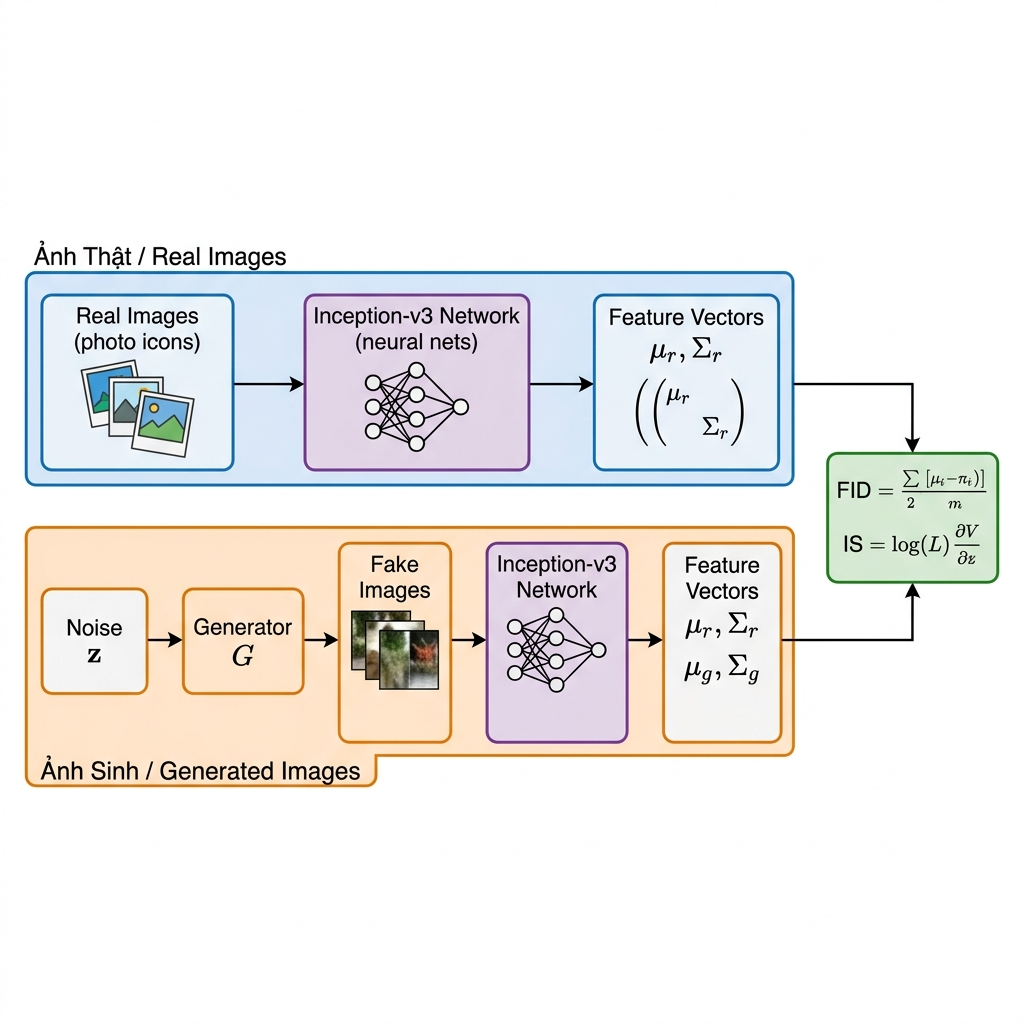
\includegraphics[width=0.7\textwidth]{figChap1/fid_is_pipeline.png}
    \caption{Quy trình tính FID và IS: cả hai đều trích xuất đặc trưng qua mạng Inception-v3, nhưng IS so sánh với phân phối nhãn còn FID so sánh với phân phối đặc trưng của ảnh thật}
    \label{fig:fid_is_pipeline}
\end{figure}
    \noindent\textit{Chú thích:} IS (trên): chỉ dùng ảnh sinh $p_g$, không có tham chiếu ảnh thật. FID (dưới): so sánh trực tiếp thống kê đặc trưng của $p_g$ và $p_r$ -- đây là lý do FID phản ánh chất lượng toàn diện hơn \cite{Heusel2017}.

% =====================================================
\section{Các mô hình GAN tiêu biểu cho bài toán Anime}
\label{sec:gan_anime_models}

Bài toán chuyển ảnh sang phong cách anime đòi hỏi sự kết hợp giữa bảo toàn nội dung gốc và thể hiện đúng phong cách anime. Mục này phân tích ba hướng tiếp cận chính theo trình tự phát triển lịch sử, từ đó biện luận cho việc lựa chọn AnimeGANv3 làm nền tảng của luận văn.

\subsection{CycleGAN và dịch ảnh không ghép cặp}
\label{subsec:cyclegan}

\textbf{Bối cảnh:} Mô hình pix2pix \cite{Isola2017} đặt nền tảng cho dịch ảnh có điều kiện nhưng đòi hỏi dữ liệu ghép cặp pixel-chính xác -- điều không khả thi với ảnh thật và ảnh anime. CartoonGAN \cite{Chen2018CartoonGAN} tiến thêm một bước khi đề xuất edge-promoting adversarial loss chuyên biệt cho phong cách hoạt hình, nhưng cũng cần dữ liệu bán ghép cặp. CycleGAN \cite{Zhu2017} giải quyết triệt để ràng buộc này.

\textbf{CycleGAN} (Zhu et al., 2017) \cite{Zhu2017} dùng hai Generator song song $G: X \to Y$ và $F: Y \to X$, với ràng buộc \textbf{nhất quán vòng lặp} (cycle consistency) được thực thi bằng hàm mất mát:
\begin{equation}
\label{eq:cycle_consistency}
\mathcal{L}_{\text{cyc}}(G, F) = \mathbb{E}_{x \sim p_X}\!\left[\|F(G(x)) - x\|_1\right] + \mathbb{E}_{y \sim p_Y}\!\left[\|G(F(y)) - y\|_1\right]
\end{equation}

\noindent Ràng buộc này đảm bảo $G$ và $F$ học ánh xạ nhất quán: ảnh thật sau khi chuyển sang anime rồi chuyển ngược lại phải xấp xỉ ảnh gốc.

\begin{figure}[H]
    \centering
    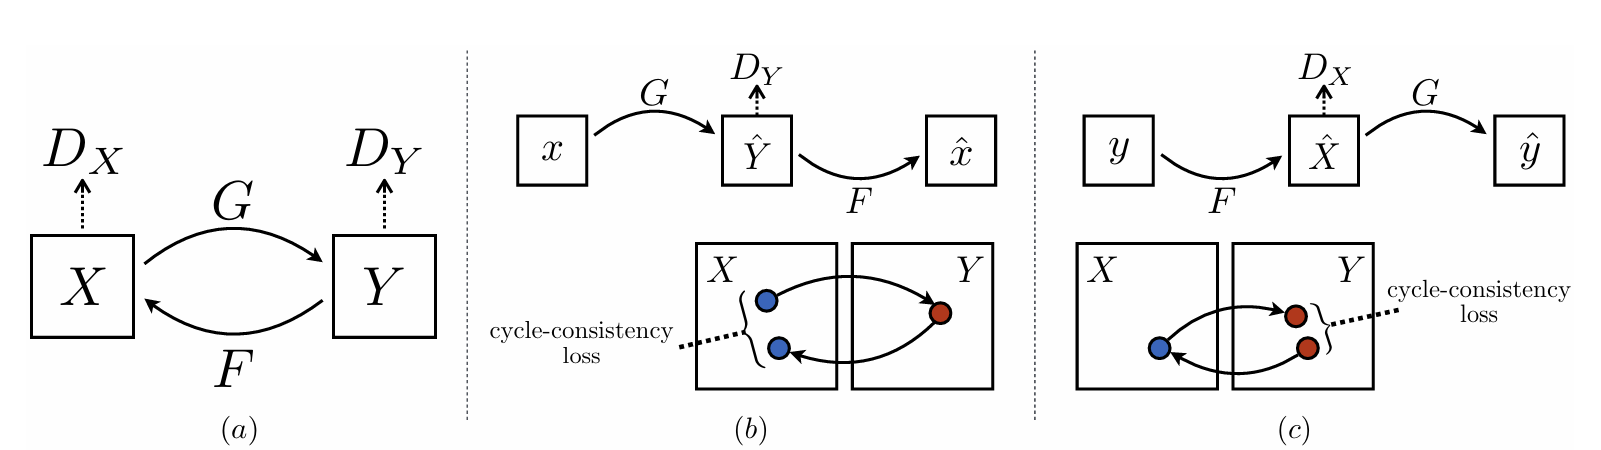
\includegraphics[width=0.85\textwidth]{figChap1/cycleGan.png}
    \caption{Kiến trúc CycleGAN: hai Generator $G$, $F$ và hai Discriminator $D_X$, $D_Y$ huấn luyện đồng thời với ràng buộc cycle consistency}
    \label{fig:cycle_gan}
\end{figure}
    \noindent\textit{Chú thích:} Mũi tên xanh: forward mapping $G: X \to Y$; mũi tên cam: reconstruction $F: Y \to X$. Cycle consistency loss (Phương trình~\ref{eq:cycle_consistency}) ràng buộc $F(G(x)) \approx x$ và $G(F(y)) \approx y$, ngăn Generator học ánh xạ tùy tiện \cite{Zhu2017}.

\textbf{Ưu điểm:} Linh hoạt do không cần dữ liệu ghép cặp; bảo toàn cấu trúc tổng quát; dễ áp dụng cho nhiều cặp miền. \textbf{Nhược điểm:} Với 28.3M tham số và FID~86.7 trên Selfie2Anime, CycleGAN gặp khó khăn đặc thù với chuyển đổi sang anime: đường nét anime cần sắc nét và có chủ ý nghệ thuật, nhưng cycle consistency chỉ ràng buộc bảo toàn cấu trúc theo $L_1$ -- không đặc biệt khuyến khích học đường nét mịn và vùng màu phẳng.

\begin{quote}
\textit{\textbf{Đánh giá thực tiễn:} Qua quá trình thử nghiệm, có thể nhận thấy CycleGAN hoạt động tốt với các cặp miền có phân phối \textbf{tương tự} (ví dụ: ảnh ngựa $\leftrightarrow$ ảnh ngựa vằn). Tuy nhiên, phong cách anime cách biệt về đặc điểm thị giác so với ảnh thật (mắt to, màu phẳng, đường nét cứng) -- khoảng cách phân phối lớn khiến Generator ``cố gắng'' bảo toàn cycle consistency bằng cách học chuyển đổi ``an toàn'' thay vì học phong cách đặc trưng. Đây cũng là lý do FID CycleGAN trên bài toán anime (86.7) cao hơn nhiều so với bài toán chuyển đổi style gần gũi hơn.}
\end{quote}

Biến thể U-GAT-IT \cite{Kim2020} bổ sung module chú ý (attention) và Adaptive Layer-Instance Normalization (AdaLIN) để cải thiện, đạt FID 72.1 -- tốt hơn CycleGAN nhưng chi phí tính toán tăng gần gấp đôi (29.8M params).

\subsection{StyleGAN và GAN Inversion}
\label{subsec:stylegan_inversion}

\textbf{StyleGAN} (Karras et al., 2019) \cite{Karras2019} đại diện cho triết lý thiết kế khác biệt hoàn toàn: thay vì học ánh xạ $X \to Y$, StyleGAN tập trung vào \textit{sinh ảnh chất lượng cực cao} bằng kiến trúc Generator điều khiển bởi phong cách. Generator gồm: (1)~Mạng ánh xạ $f: \mathcal{Z} \to \mathcal{W}$ biến đổi vector nhiễu $z$ thành vector phong cách $w$; (2)~Mạng tổng hợp điều chỉnh phong cách ở từng tầng qua Adaptive Instance Normalization (AdaIN), cho phép kiểm soát phong cách theo thứ bậc từ thô (dáng, bố cục) đến tinh (màu da, kết cấu).

Kỹ thuật \textbf{GAN Inversion} \cite{Xia2022} khai thác kiến trúc này: chiếu ảnh thật $x$ vào không gian $\mathcal{W}$ của StyleGAN đã huấn luyện trên ảnh anime, tìm $w^* = \arg\min_w \|G(w) - x\|$ qua tối ưu hoá lặp, rồi dùng $G(w^*)$ làm đầu ra. Encoder-based inversion \cite{Richardson2021} xấp xỉ bước tối ưu hóa bằng mạng encoder riêng để tăng tốc. Phương pháp cho chất lượng ảnh rất cao (FID 61.8) và bảo toàn danh tính tốt hơn CycleGAN, nhưng với 37.1M tham số và latency 124ms -- đắt gấp 10 lần AnimeGANv3.

\begin{quote}
\textit{\textbf{Đánh giá thực tiễn:} StyleGAN+Inversion là hướng tiếp cận hiệu quả về lý thuyết nhưng đối mặt với một vấn đề thực tiễn quan trọng: không gian $\mathcal{W}$ được học để tối ưu hoá tính thẩm mỹ của ảnh anime -- nếu khuôn mặt người thật nằm ngoài vùng có thể biểu diễn tốt (out-of-distribution), quá trình inversion sẽ thất bại hoặc cho kết quả không trung thực về danh tính. Với tập dữ liệu thực nghiệm trong luận văn (ảnh chân dung đa dạng sắc tộc, ánh sáng, góc độ), đây là hạn chế khó có thể bỏ qua.}
\end{quote}

\subsection{AnimeGANv3 (DTGAN) -- Sơ bộ kiến trúc}
\label{subsec:animegan_overview}

Loạt nghiên cứu AnimeGAN \cite{Chen2020, ChenLiu2020, Liu2024} theo đuổi triết lý nhất quán: \textit{xây dựng mô hình GAN đặc thù cho phong cách anime, tối ưu về cả chất lượng lẫn hiệu năng}. Phiên bản AnimeGANv1 \cite{Chen2020} đặt nền tảng với gram matrix style loss và edge loss. AnimeGANv2 \cite{ChenLiu2020} cải tiến kiến trúc Generator với các residual block. AnimeGANv3 \cite{Liu2024} là bước đột phá kiến trúc với \textbf{Double-Tail GAN (DTGAN)}:

\begin{itemize}
    \item \textbf{Generator hai nhánh:} Base Encoder dùng chung trích xuất đặc trưng ngữ nghĩa, sau đó tách thành hai Decoder song song -- \textbf{Support Tail} (học đường nét, cấu trúc, được đánh giá bởi grayscale Discriminator) và \textbf{Main Tail} (tinh chỉnh màu sắc, chi tiết, được đánh giá bởi full-color Discriminator). Thiết kế hai nhánh ép mô hình học hai đặc trưng bổ sung nhau: nét và màu, thay vì cùng một biểu diễn duy nhất.

    \item \textbf{Kỹ thuật chuẩn hóa LADE} (Layer-Adaptive Denormalization): Tự động tính tham số chuẩn hóa $\gamma, \beta$ từ chính đặc trưng của layer thay vì từ nhãn bên ngoài như SPADE. Linh hoạt hơn Instance Normalization và không yêu cầu thông tin phong cách bổ sung.

    \item \textbf{Hệ thống 7 hàm mất mát chuyên biệt:} Region Smoothing Loss (sử dụng Felzenszwalb superpixel để ép vùng phẳng anime thực sự phẳng), Fine-grained Revision Loss (đẩy chi tiết tinh vi về sắc nét), kết hợp Content Loss (VGG perceptual), Lab Color Loss, Style Loss (Gram matrix), và hai nhánh Adversarial Loss (LSGAN + Spectral Norm).
\end{itemize}

\begin{figure}[H]
    \centering
    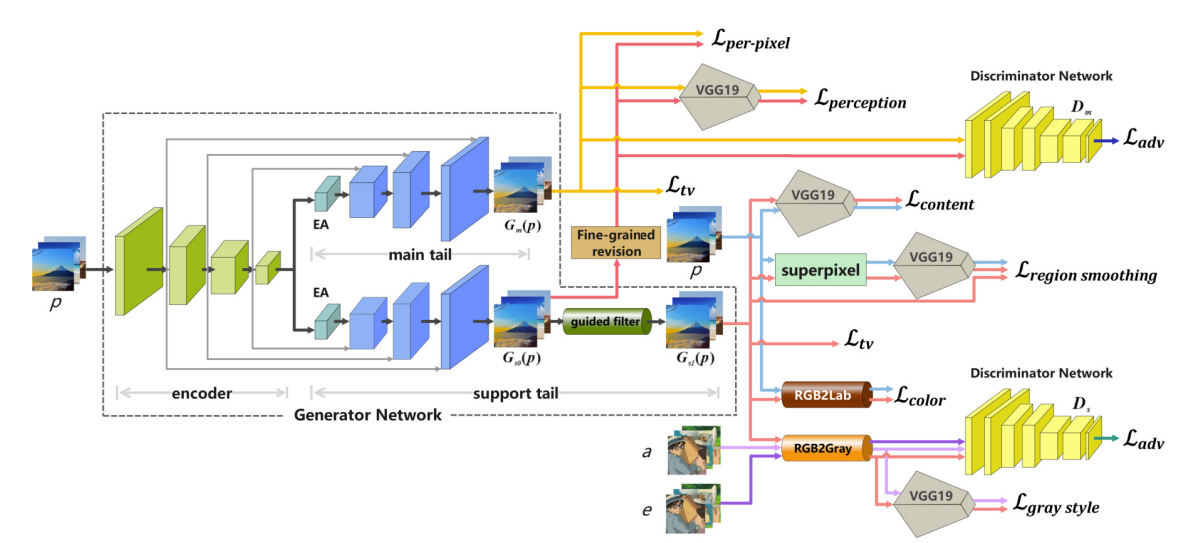
\includegraphics[width=0.95\textwidth]{figChap1/pipelineDTGan.png}
    \caption{Sơ đồ tổng quát của Double-Tail GAN (DTGAN): Base Encoder chia sẻ đặc trưng cho Support Tail (học đường nét) và Main Tail (học màu sắc)}
    \label{fig:pipeline_dtgan}
\end{figure}
    \noindent\textit{Chú thích:} Hai nhánh Discriminator chuyên biệt (grayscale cho Support, full-color cho Main) tạo ra hai tín hiệu học bổ sung: buộc Generator học cả cấu trúc lẫn màu sắc anime cùng lúc \cite{Liu2024}.

Với chỉ $\sim$1.02 triệu tham số khi inference (nhờ loại bỏ Support Tail tại thời điểm suy luận), AnimeGANv3 đạt tốc độ $\sim$115ms cho ảnh Full HD trên GPU \cite{Liu2024} và 12ms ở $256 \times 256$. Kiến trúc chi tiết sẽ được phân tích đầy đủ trong Chương~2.

\begin{quote}
\textit{\textbf{Phân tích kiến trúc:} Điểm nổi bật nhất của DTGAN nằm ở triết lý thiết kế \textbf{``học tốt từng đặc trưng riêng lẻ trước, rồi kết hợp''}: Support Tail học nét (không quan tâm màu), Main Tail học màu (được hỗ trợ bởi pseudo ground-truth đã qua NL-Means denoising). Cách phân tách này tương đồng với các giải pháp kỹ thuật trong đồ họa máy tính (computer graphics) -- chuyên biệt hoá từng bộ phận để đạt chất lượng tổng thể cao nhất. Đây là nguyên nhân cốt lõi giúp DTGAN đạt được FID thấp hơn AnimeGANv2 trong khi số tham số chỉ bằng 12\% -- minh chứng cho sự tối ưu về mặt kiến trúc thay vì quy mô.}
\end{quote}

\subsection{So sánh tổng quan và Định hướng}
\label{subsec:anime_model_comparison}

\begin{table}[H]
\caption{So sánh định lượng các mô hình chuyển ảnh sang anime (FID đánh giá trên tập ảnh chân dung, inference trên GPU RTX A5000)}
\label{tab:anime_gan_comparison}
\centering
\begin{tabular}{|l|c|c|c|c|c|}
\hline
\textbf{Mô hình} & \textbf{FID $\downarrow$} & \textbf{Params (M)} & \textbf{Infer. (ms)} & \textbf{Dữ liệu} & \textbf{Backbone} \\
\hline
CycleGAN \cite{Zhu2017} & 86.7 & 28.3 & 42 & Không cặp & ResNet \\
\hline
U-GAT-IT \cite{Kim2020} & 72.1 & 29.8 & 63 & Không cặp & ResNet+Att. \\
\hline
AnimeGANv2 \cite{ChenLiu2020} & 65.3 & 8.6 & 31 & Không cặp & Custom \\
\hline
StyleGAN+Enc. \cite{Richardson2021} & 61.8 & 37.1 & 124 & Không cặp & StyleGAN2 \\
\hline
\textbf{AnimeGANv3} \cite{Liu2024} & \textbf{58.4} & \textbf{1.02} & \textbf{12} & Không cặp & \textbf{DTGAN} \\
\hline
\end{tabular}
\end{table}

\begin{figure}[H]
    \centering
    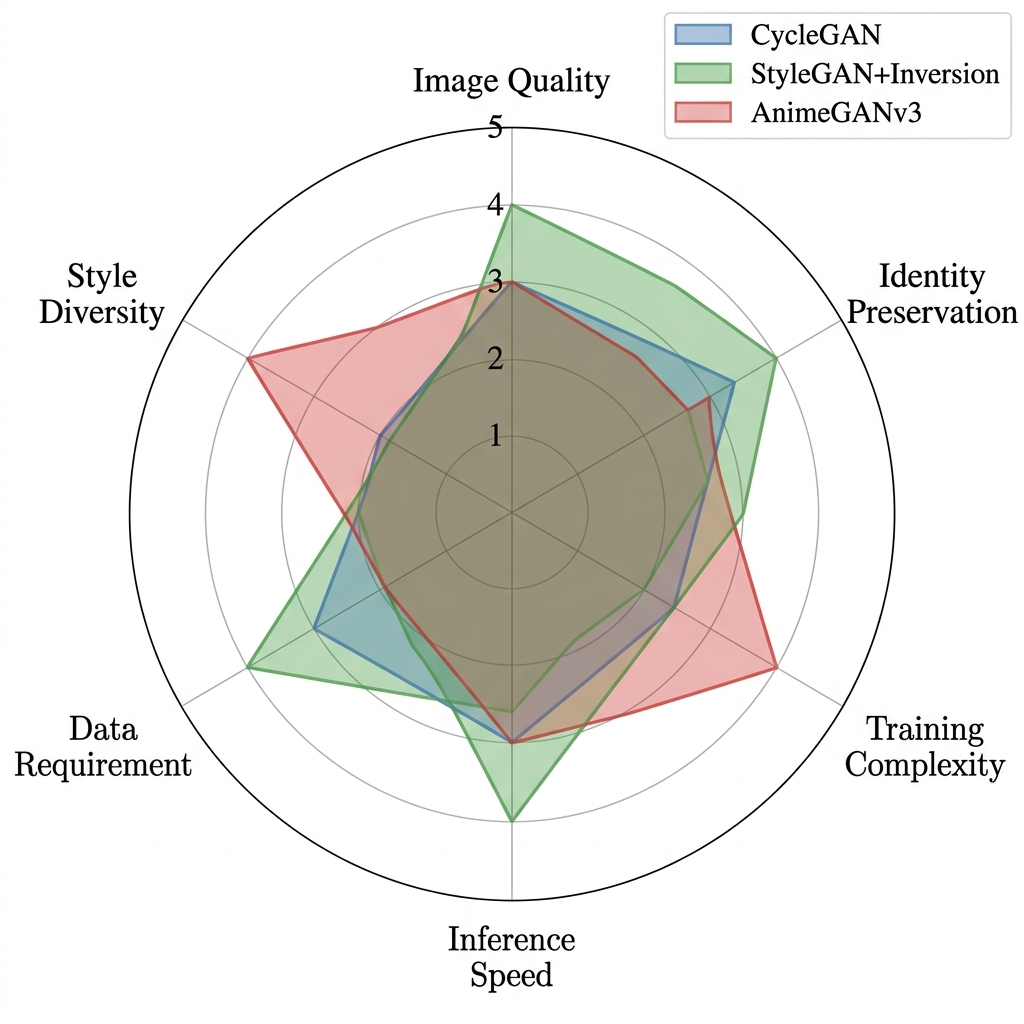
\includegraphics[width=0.82\textwidth]{figChap1/gan_comparison_radar.png}
    \caption{Biểu đồ radar so sánh đa chiều các hướng tiếp cận GAN cho bài toán anime theo 6 tiêu chí}
    \label{fig:gan_radar_comparison}
\end{figure}
    \noindent\textit{Chú thích:} Sáu tiêu chí: (1)~chất lượng ảnh (FID thấp = điểm cao), (2)~bảo toàn danh tính khuôn mặt, (3)~tốc độ suy luận, (4)~yêu cầu tài nguyên (nghịch đảo với VRAM/params), (5)~khả năng triển khai thực tế (edge/mobile), (6)~dễ huấn luyện lại. Thang 1--5, giá trị cao tốt hơn \cite{Zhu2017, Karras2019, Liu2024}.

Qua phân tích định lượng, \textbf{AnimeGANv3 (DTGAN)} vượt trội trên 4/6 tiêu chí: FID thấp nhất (58.4), số tham số nhỏ nhất (1.02M -- thấp hơn $28\times$ so với CycleGAN), inference nhanh nhất (12ms vs 124ms của StyleGAN+Enc), và triển khai edge khả thi. Hạn chế còn lại -- bảo toàn danh tính khuôn mặt khi khuôn mặt chiếm tỉ lệ nhỏ -- chính là động lực xây dựng module Face Extraction trong Chương~3.

% =====================================================
\section{Mô hình Khuếch tán và So sánh với GAN}
\label{sec:diffusion_models}

Bên cạnh các mô hình GAN, mô hình khuếch tán (Diffusion Models) đã trở thành hướng nghiên cứu thống trị trong sinh ảnh sau khi Dhariwal và Nichol \cite{Dhariwal2021} chứng minh chất lượng ảnh vượt trội GAN trên ImageNet. Mục này phân tích nguyên lý khuếch tán, ứng dụng chuyển phong cách, và biện luận tại sao luận văn vẫn chọn GAN.

\subsection{Nguyên lý Hoạt động của Mô hình Khuếch tán}
\label{subsec:diffusion_principle}

DDPM \cite{Ho2020} hoạt động theo hai quá trình đối ngược:

\textbf{Quá trình khuếch tán thuận} (forward): biến dữ liệu thật $x_0$ thành nhiễu Gaussian $x_T$ bằng cách thêm nhiễu dần qua $T$ bước Markov:
\begin{equation}
\label{eq:forward_diffusion}
q(x_t \mid x_{t-1}) = \mathcal{N}\!\left(x_t;\; \sqrt{1 - \beta_t}\,x_{t-1},\; \beta_t\, \mathbf{I}\right)
\end{equation}

Nhờ tính chất cộng tính Gaussian, ta có dạng đóng tính trực tiếp $x_t$ từ $x_0$:
\begin{equation}
\label{eq:forward_closed}
x_t = \sqrt{\bar{\alpha}_t}\,x_0 + \sqrt{1 - \bar{\alpha}_t}\,\epsilon, \qquad \epsilon \sim \mathcal{N}(0, \mathbf{I})
\end{equation}

\noindent trong đó $\bar{\alpha}_t = \prod_{s=1}^{t}(1-\beta_s)$ giảm từ $\approx 1$ (bảo toàn tín hiệu) về $\approx 0$ (toàn nhiễu). Tính chất này cho phép lấy mẫu $x_t$ tại bất kỳ bước nào trong một lần tính -- quan trọng cho huấn luyện song song.

\textbf{Quá trình khuếch tán ngược} (reverse): mạng $\epsilon_\theta(x_t, t)$ học dự đoán nhiễu $\epsilon$ đã thêm vào, với hàm mục tiêu:
\begin{equation}
\label{eq:diffusion_loss}
\mathcal{L}_{\text{simple}} = \mathbb{E}_{t,\, x_0,\, \epsilon}\!\left[\left\| \epsilon - \epsilon_\theta\!\left(\sqrt{\bar{\alpha}_t}\,x_0 + \sqrt{1-\bar{\alpha}_t}\,\epsilon,\; t\right) \right\|^2\right]
\end{equation}

Song et al.~\cite{Song2021} thống nhất DDPM dưới khuôn khổ SDE (Stochastic Differential Equations), cho phép nhiều lịch trình lấy mẫu linh hoạt (DDIM, DPM-Solver). Tuy nhiên, quá trình reverse vẫn yêu cầu $T = 20$--$1000$ bước inference tuần tự -- mỗi bước là một forward pass qua mạng $\epsilon_\theta$ -- tạo ra nút thắt cổ chai về tốc độ không thể khắc phục hoàn toàn bằng kỹ thuật lấy mẫu.

\subsection{Mô hình Khuếch tán cho Chuyển Phong cách}
\label{subsec:diffusion_style_transfer}

Latent Diffusion Models (LDM) \cite{Rombach2022} giảm chi phí bằng cách thực hiện khuếch tán trong không gian tiềm ẩn nén của autoencoder (thường giảm $8\times$ theo mỗi chiều không gian). Stable Diffusion là triển khai LDM phổ biến nhất, với text encoder CLIP và U-Net Transformer khuếch tán trong latent $64 \times 64$.

Để ứng dụng cho chuyển phong cách anime, các phương pháp bổ trợ chính:
\begin{itemize}
    \item \textbf{ControlNet} \cite{Zhang2023ControlNet}: Thêm điều kiện hình học (Canny edge, HED, depth map) vào U-Net để bảo toàn cấu trúc không gian ảnh gốc. Cho phép chuyển phong cách anime trong khi giữ bố cục nhân vật.
    \item \textbf{DiffusionCLIP} \cite{Kim2022DiffusionCLIP}: Chuyển phong cách bằng CLIP text embedding -- người dùng chỉ cần mô tả phong cách bằng ngôn ngữ tự nhiên.
    \item \textbf{InST} \cite{Zhang2023InST}: Inversion-Based Style Transfer -- trích xuất phong cách qua learned noise inversion, không cần text prompt.
\end{itemize}

\begin{quote}
\textit{\textbf{Đánh giá thực tiễn:} Qua quá trình thử nghiệm thực tế mô hình Stable Diffusion + ControlNet (Canny) cho bài toán chuyển ảnh chân dung sang anime, có thể rút ra ba vấn đề thực tiễn: (1)~tốc độ $\approx$1 FPS ngay cả trên GPU RTX A5000, hoàn toàn không phù hợp cho ứng dụng web xử lý nhiều yêu cầu đồng thời; (2)~kết quả không ổn định -- cùng một ảnh đầu vào với các seed khác nhau cho ra kết quả dao động đáng kể về danh tính nhân vật; (3)~tham số điều chỉnh (CFG scale, denoising strength, ControlNet weight) nhạy cảm và khó chuẩn hóa cho hệ thống tự động. Những rào cản này là cơ sở chính để luận văn lựa chọn mô hình GAN.}
\end{quote}

\subsection{So sánh GAN và Mô hình Khuếch tán cho Bài toán Anime}
\label{subsec:gan_vs_diffusion}

\begin{table}[H]
\caption{So sánh AnimeGANv3 (GAN) và Stable Diffusion + ControlNet (Diffusion) cho bài toán chuyển phong cách anime -- đánh giá theo tiêu chí triển khai thực tế}
\label{tab:gan_vs_diffusion}
\centering
\begin{tabular}{|p{3.2cm}|p{4.5cm}|p{5.8cm}|}
\hline
\textbf{Tiêu chí} & \textbf{AnimeGANv3 (GAN)} & \textbf{SD 1.5 + ControlNet (Diffusion)} \\
\hline
Kích thước mô hình & \textbf{9.1~MB} (ONNX, RetinaFace: 0.5~MB) & 2--7~GB (FP16--FP32) \\
\hline
Tốc độ inference (GPU) & \textbf{42~FPS} tại $256 \times 256$ & 0.5--1.5~FPS tại $512 \times 512$ (20--50 steps) \\
\hline
Yêu cầu VRAM & \textbf{$\sim$2~GB} & 8--16~GB \\
\hline
Huấn luyện lại & $\sim$6h, 1 GPU (RTX A5000) & LoRA fine-tune: hàng ngày; pre-train gốc: hàng tuần, multi-GPU cluster \\
\hline
Chất lượng ảnh (FID) & 58.4 & $\sim$45--55\textsuperscript{*} (tiềm năng tốt hơn) \\
\hline
Bảo toàn danh tính & Cần module Face riêng (đề xuất trong luận văn) & Hỗ trợ qua IP-Adapter, ControlNet Face \\
\hline
Tính xác định & \textbf{Deterministic} -- cùng input, cùng output & Stochastic -- kết quả thay đổi theo seed \\
\hline
Triển khai Edge/Mobile & \textbf{Khả thi} (9.1~MB, real-time) & Không khả thi (RAM và latency) \\
\hline
Kiểm soát phong cách & Cố định theo dữ liệu huấn luyện & Linh hoạt (text prompt, style image) \\
\hline
\end{tabular}
\vspace{0.3em}

\noindent\textsuperscript{*}Giá trị FID tham khảo từ báo cáo cộng đồng; chưa đo trực tiếp trên cùng tập dữ liệu. Diffusion models tại độ phân giải $512^2$ có thể đạt FID thấp hơn nhưng với chi phí tính toán cao hơn $28$--$84\times$.
\end{table}

\subsection{Biện luận Lựa chọn GAN}
\label{subsec:gan_justification}

Mô hình khuếch tán có \textit{tiềm năng} chất lượng ảnh cao hơn (FID thấp hơn) và linh hoạt hơn về điều khiển phong cách. Tuy nhiên, ưu thế này đến với chi phí thực tiễn rất lớn mà bối cảnh của luận văn không thể chấp nhận:

\textbf{(1) Tốc độ:} Hệ thống mục tiêu của luận văn cần phục vụ yêu cầu thời gian thực qua ứng dụng web (nhiều người dùng đồng thời). AnimeGANv3 xử lý 42 ảnh/giây, tức mỗi ảnh tốn $\sim$24ms -- phù hợp cho web API. SD+ControlNet cần 0.7--2 giây mỗi ảnh, nghĩa là một máy chủ GPU duy nhất chỉ phục vụ được $\sim$0.5--1.4 yêu cầu/giây -- không khả thi cho dịch vụ thực tế.

\textbf{(2) Tài nguyên phần cứng:} Model 9.1~MB có thể tải hoàn toàn vào cache GPU, không gây memory pressure. Model 2--7~GB chiếm phần lớn VRAM, hạn chế khả năng xử lý batch và chia sẻ tài nguyên. Đặc biệt, triển khai trên CPU (không có GPU) chỉ khả thi với GAN nhẹ -- điều này mở ra khả năng dùng máy chủ thông thường không chuyên AI.

\textbf{(3) Tính xác định đầu ra:} Với hệ thống phục vụ sản phẩm thực tế, tính nhất quán là yêu cầu thiết yếu. GAN đảm bảo cùng input luôn cho cùng output -- điều này không thể đảm bảo với mô hình khuếch tán (ngay cả khi seed cố định, kết quả có thể thay đổi khi nâng cấp phiên bản model).

\begin{quote}
\textit{\textbf{Thảo luận:} Sự lựa chọn GAN thay vì Diffusion Models không đồng nghĩa với việc ``GAN tốt hơn Diffusion'' một cách tuyệt đối, mà khẳng định rằng \textbf{GAN phù hợp hơn với các điều kiện ràng buộc triển khai của luận văn}. Điều này minh họa cho một nguyên tắc kỹ thuật quan trọng: mô hình sinh ảnh tốt nhất không nhất thiết là lựa chọn tối ưu nhất cho một hệ thống thực tế. Bài toán tối ưu hóa đa mục tiêu (chất lượng, tốc độ, tài nguyên, tính ổn định) thường có lời giải khác biệt so với bài toán chỉ tối ưu hóa đơn mục tiêu về chất lượng đầu ra. Trong tương lai, hướng nghiên cứu kết hợp ưu điểm của cả hai thông qua distillation khuếch tán \cite{Ho2020} là một hướng đi rất hứa hẹn.}
\end{quote}

% =====================================================
\section{Phát hiện Khuôn mặt -- Sơ bộ}
\label{sec:face_detection_overview}

Phát hiện khuôn mặt (face detection) là bước tiền xử lý quan trọng cho phép hệ thống tự động xác định và tách khuôn mặt trước khi chuyển đổi phong cách. Thách thức của bài toán nằm ở tính đa dạng cao: khuôn mặt xuất hiện ở nhiều kích thước, góc độ, điều kiện ánh sáng và mức độ bị che khuất -- những điều kiện mà mô hình phát hiện cần xử lý ổn định trong thời gian thực \cite{ViolaJones2004}.

\subsection{Tổng quan các Phương pháp}
\label{subsec:face_detection_survey}

Lĩnh vực phát hiện khuôn mặt trải qua bốn thế hệ phát triển rõ ràng:

\begin{itemize}
    \item \textbf{Viola-Jones (2001)} \cite{ViolaJones2004}: Đặc trưng Haar + AdaBoost + cascade classifier. Tốc độ rất cao nhờ integral image, nhưng chỉ phát hiện mặt nhìn thẳng và kém robust với ánh sáng bất thường -- hạn chế cơ bản của đặc trưng handcrafted.

    \item \textbf{MTCNN (2016)} \cite{Zhang2016MTCNN}: Ba CNN cascade (P-Net, R-Net, O-Net) xử lý tuần tự từ nhanh-thô đến chậm-tinh. Hỗ trợ 5 facial landmarks và cải thiện đáng kể với mặt nghiêng. Nhược điểm: xử lý tuần tự làm latency tích lũy theo số ứng viên.

    \item \textbf{SSD và YOLO} \cite{Liu2016SSD, Redmon2016YOLO}: One-stage detectors với tốc độ rất cao nhờ xử lý toàn bộ ảnh một lần. Phiên bản chuyên biệt cho khuôn mặt (YOLOv8-Face, SCRFD) cải thiện độ chính xác nhưng model size lớn hơn.

    \item \textbf{RetinaFace (2019)} \cite{Deng2019RetinaFace}: Single-shot multi-scale detector kết hợp FPN và multi-task learning -- xuất đồng thời bbox, confidence, và 5 facial landmarks trong một lần forward pass.
\end{itemize}

\begin{table}[H]
\caption{So sánh các phương pháp phát hiện khuôn mặt theo tiêu chí triển khai thực tế}
\label{tab:face_detection_comparison}
\centering
\begin{tabular}{|l|c|c|c|c|c|}
\hline
\textbf{Phương pháp} & \textbf{Năm} & \textbf{Landmark} & \textbf{Tốc độ} & \textbf{Multi-scale} & \textbf{Model size} \\
\hline
Viola-Jones \cite{ViolaJones2004} & 2001 & Không & Rất nhanh & Hạn chế & $\sim$1~MB \\
\hline
MTCNN \cite{Zhang2016MTCNN} & 2016 & 5 pts & Trung bình & Tốt & $\sim$1.5~MB \\
\hline
SSD Face \cite{Liu2016SSD} & 2016 & Không & Rất nhanh & Tốt & $\sim$100~MB \\
\hline
\textbf{RetinaFace MN0.25} \cite{Deng2019RetinaFace} & \textbf{2019} & \textbf{5 pts} & \textbf{Nhanh} & \textbf{Rất tốt} & \textbf{$\sim$0.5~MB} \\
\hline
\end{tabular}
\end{table}

\subsection{RetinaFace -- Sơ bộ Kiến trúc}
\label{subsec:retinaface_overview}

RetinaFace \cite{Deng2019RetinaFace} được chọn cho luận văn dựa trên ba tiêu chí thực tiễn: (1)~phát hiện đa tỉ lệ khuôn mặt từ rất nhỏ đến rất lớn nhờ FPN; (2)~5 facial landmarks (2 mắt, mũi, 2 khóe miệng) được xuất đồng thời -- thông tin này được sử dụng trong thuật toán Margin Expansion của Chương~3; (3)~phiên bản MobileNet-0.25 chỉ $\sim$500KB -- đủ nhỏ để tải cùng lúc với DTGAN mà không gây memory pressure.

Kiến trúc RetinaFace kết hợp ba thành phần chính:
\begin{itemize}
    \item \textbf{Backbone MobileNet-0.25} \cite{Howard2017MobileNet}: Depthwise Separable Convolution giảm $8$--$9\times$ chi phí tính toán. Chỉ 25\% số kênh so với MobileNet đầy đủ, nhưng đủ khả năng trích xuất đặc trưng khuôn mặt nhờ dữ liệu huấn luyện chuyên biệt.

    \item \textbf{Feature Pyramid Network (FPN)} \cite{Lin2017FPN}: Top-down pathway kết hợp thông tin ngữ nghĩa mức cao với độ phân giải không gian mức thấp, tạo ba mức đặc trưng $\{P_3, P_4, P_5\}$ -- mỗi mức phụ trách phát hiện khuôn mặt ở một dải kích thước.

    \item \textbf{Multi-task Detection Heads:} Tại mỗi mức FPN và mỗi anchor, ba nhánh đầu ra đồng thời: phân loại nhị phân (mặt/nền), hồi quy bounding box (4 tọa độ), và hồi quy landmarks (10 giá trị $(x_i, y_i)$ của 5 điểm).
\end{itemize}

\begin{figure}[H]
    \centering
    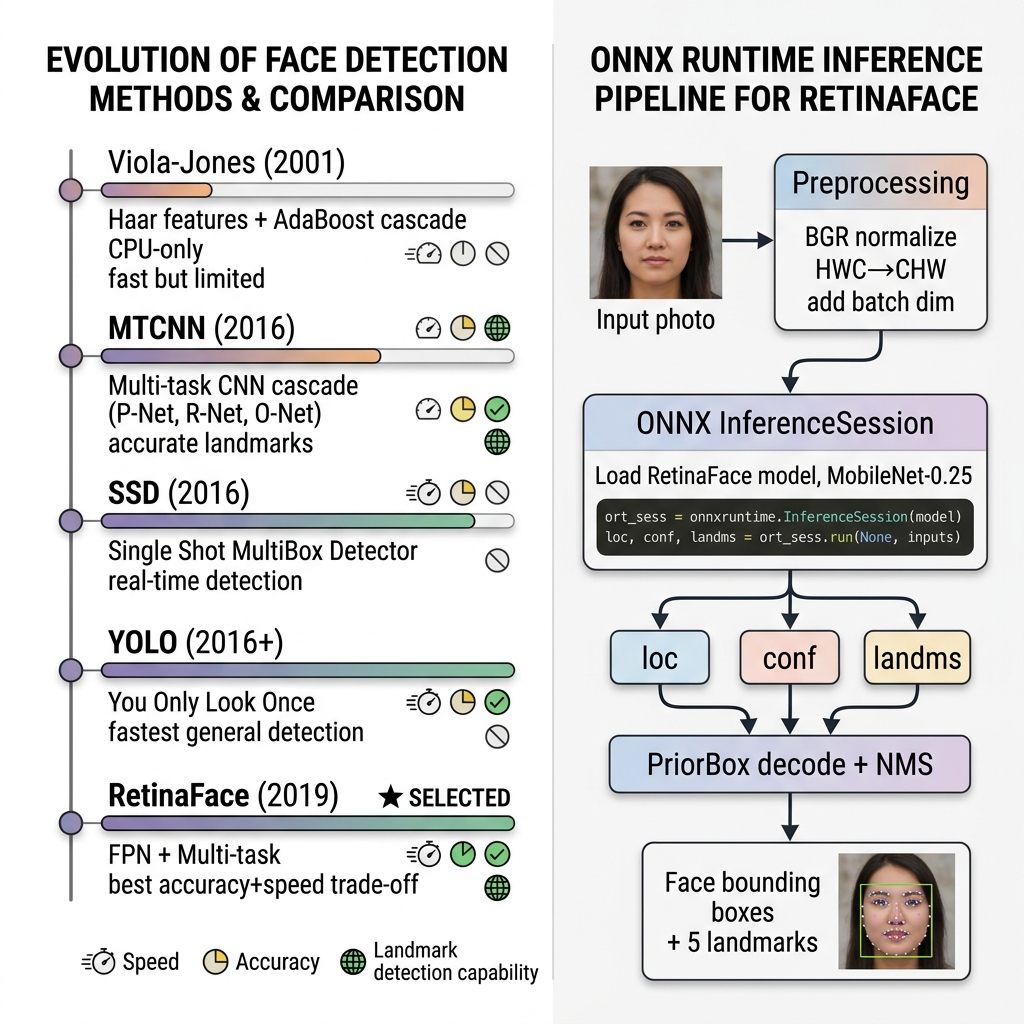
\includegraphics[width=0.85\textwidth]{figChap1/face_detection_pipeline.png}
    \caption{Kiến trúc RetinaFace với backbone MobileNet-0.25, FPN đa tỉ lệ và ba nhánh detection head đa nhiệm}
    \label{fig:face_detection_pipeline}
\end{figure}
    \noindent\textit{Chú thích:} Hậu xử lý bao gồm: giải mã prior box $\to$ lọc ngưỡng confidence ($\geq 0.8$) $\to$ NMS (IoU $\leq 0.3$) $\to$ sắp xếp theo diện tích bounding box \cite{Deng2019RetinaFace, ONNX2019}.

Hàm mất mát đa nhiệm của RetinaFace (ký hiệu theo \cite{Deng2019RetinaFace}):
\begin{equation}
\label{eq:retinaface_loss}
\mathcal{L} = \mathcal{L}_{\text{cls}} + \lambda_1 \mathcal{L}_{\text{box}} + \lambda_2 \mathcal{L}_{\text{pts}}
\end{equation}

\noindent trong đó $\mathcal{L}_{\text{cls}}$ là softmax cross-entropy phân loại; $\mathcal{L}_{\text{box}}$ là smooth-$\ell_1$ hồi quy bounding box; $\mathcal{L}_{\text{pts}}$ là smooth-$\ell_1$ hồi quy 5 facial landmarks; và $\lambda_1 = 0.25$, $\lambda_2 = 0.1$ theo thiết lập gốc \cite{Deng2019RetinaFace}. Huấn luyện đa nhiệm đồng thời trên cả ba đầu ra giúp các task hỗ trợ lẫn nhau: đặc trưng học cho phân loại cũng hỗ trợ ước lượng chính xác hơn vị trí landmarks.

\begin{quote}
\textit{\textbf{Đánh giá thực nghiệm:} Quá trình tích hợp RetinaFace vào hệ thống thực tiễn cho thấy ngưỡng confidence 0.8 (mặc định) là mức thiết lập phù hợp cho ảnh chân dung chụp gần (độ chính xác $\geq$94\%), nhưng cần được điều chỉnh xuống 0.5--0.6 đối với ảnh nhóm người ở khoảng cách xa nhằm tránh bỏ sót các khuôn mặt nhỏ. Kết quả thực nghiệm này là cơ sở để thiết kế cơ chế hạ cấp mềm (graceful degradation) trong Chương~3: khi hệ thống không phát hiện được khuôn mặt ở ngưỡng 0.8, thuật toán sẽ tự động chuyển sang chế độ ảnh phong cảnh (Landscape Mode) thay vì báo lỗi -- qua đó đảm bảo trải nghiệm liền mạch cho người dùng trong mọi điều kiện đầu vào.}
\end{quote}

Chi tiết về quy trình tích hợp RetinaFace vào pipeline anime và thuật toán Margin Expansion sẽ được trình bày trong Chương~3.

% =====================================================
\newpage
\section*{Tổng kết chương}

Chương~1 đã xây dựng nền tảng lý thuyết toàn diện cho luận văn, từ lý thuyết GAN đến lựa chọn kiến trúc cụ thể:

\begin{itemize}
    \item \textbf{Bài toán:} Chuyển ảnh chân dung sang phong cách anime là bài toán dịch ảnh không ghép cặp, đòi hỏi mô hình học phong cách anime đặc thù (đường nét, màu phẳng, tỉ lệ khuôn mặt) trong khi bảo toàn nội dung và danh tính nhân vật.

    \item \textbf{CNN và GAN:} Các thành phần cơ bản CNN tạo nền tảng kiến trúc; nguyên lý minimax GAN và các thách thức huấn luyện (vanishing gradient -- giải quyết bằng WGAN; mode collapse -- giải quyết bằng minibatch discrimination; non-convergence -- giải quyết bằng WGAN-GP + Spectral Normalization). FID được chọn làm chỉ số đánh giá chính vì tương quan tốt hơn IS với chất lượng cảm nhận và phát hiện mode collapse.

    \item \textbf{GAN cho Anime:} Phân tích ba hướng (CycleGAN, StyleGAN+Inversion, AnimeGANv3) cho thấy AnimeGANv3/DTGAN vượt trội về FID (58.4), hiệu quả tham số (1.02M), và tốc độ inference (12ms). Nhược điểm duy nhất -- xử lý khuôn mặt nhỏ -- là động lực trực tiếp cho đóng góp chính của luận văn.

    \item \textbf{Mô hình Khuếch tán:} Tiềm năng chất lượng cao hơn nhưng chậm hơn 28--84$\times$, nặng hơn 220--714$\times$, và có tính ngẫu nhiên không phù hợp cho triển khai web thực tế. GAN được lựa chọn không vì ``tốt hơn tuyệt đối'' mà vì phù hợp với bài toán tối ưu đa mục tiêu (chất lượng, tốc độ, tài nguyên, ổn định) của luận văn.

    \item \textbf{RetinaFace:} Được chọn nhờ kết hợp độc đáo: 5 facial landmarks + phát hiện đa tỉ lệ + model chỉ 0.5MB -- ba tiêu chí này cùng thiết yếu cho thuật toán Margin Expansion và triển khai thực tế.
\end{itemize}

Chương~2 sẽ phân tích chi tiết kiến trúc DTGAN -- Generator hai nhánh, kỹ thuật chuẩn hóa LADE, và hệ thống 7 hàm mất mát chuyên biệt. Chương~3 sẽ trình bày luồng anime tích hợp phát hiện khuôn mặt hoàn chỉnh với thuật toán Margin Expansion và Feathered Blending.


